\section{Simulator Architecture, Model Ladder, and Experimental Protocols}\label{app:repro}

\begin{figure}[tbp]
\centering
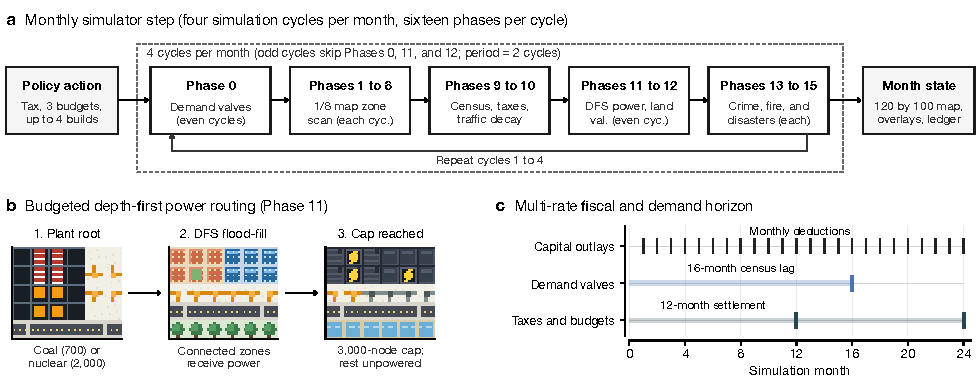
\includegraphics[width=\textwidth]{figures/fig_anatomy.pdf}
\caption{\textbf{Internal monthly execution anatomy of the Micropolis C++ engine.} Constants shown are verified programmatically against the simulator source tree before rendering. \textbf{a}, Each monthly step applies the policy instruments, executes four simulation cycles of sixteen deterministic phases at speed \ProtoSpeed{} (ordered sequentially from phase zero to phase fifteen; even cycles update R/C/I demand valves, global DFS power routing, and pollution/land-value fields; each cycle scans one eighth of the \WorldW{}-by-\WorldH{} map West-to-East and updates transport decay, crime, population density, fire coverage, and stochastic disasters; monthly census totals update each four-cycle month and annual taxes settle at forty-eight-cycle intervals), and reads the resulting state. \textbf{b}, Power distribution uses a budgeted depth-first flood-fill over conductive tiles starting from active coal and nuclear plants pushed onto the scan stack; once plant tile budgets or stack pointers run out, downstream zones lose power (illustrated across three procedural micro-sprite stages). \textbf{c}, Non-local temporal coupling over a \Horizon-month plan, where construction outlays deduct immediately each month from reserves, R/C/I demand valves refresh on sixteen-month census horizons, and annual tax receipts minus service budgets settle once a year.}
\label{fig:anatomy}
\end{figure}

\subsection{Exact Simulator and Deterministic Replay}\label{app:engine}

Micropolis couples cellular-automaton spatial updates to global resource constraints spanning budgeted depth-first power routing, annual fiscal accounting, and census-driven R/C/I demand valves (Figure~\ref{fig:anatomy}). We drive the C++ core exclusively through clean episode resets that load a starting city file, set the disasters flag, read the initial observation, seed the internal PRNG once, and apply each month's tax rate, three service funding ratios, ordered spatial tool calls, and any scheduled task event before stepping four city-time units at speed \ProtoSpeed{} (one pass per tick, easy game level, auto-budget and auto-bulldoze active). Three upstream non-determinism bugs were patched and documented in the C++ source tree (an uninitialised callback pointer, heap-allocated sprite name strings, and wall-clock PRNG reseeding on map loads). Genuine simulator mechanics (including traversal-order power allocation and branch dropping when the DFS stack fills) are preserved untouched so world models face the true dynamics.

Across all \OracleCities{} bundled cities stepped for \OracleMonths{} months with stochastic disasters enabled, full-state hashes match identically at each month across fresh processes, previously dirtied simulator instances, and two independent host architectures. The structured state exposed to the world model comprises the \WorldW{}-by-\WorldH{} tile-code grid, native-resolution spatial overlays, twenty municipal scalars, and a carry-over bookkeeping ledger of \LedgerEntries{} entries plus two auxiliary maps. Restoring this observation alongside PRNG and active-sprite state reproduces the subsequent twelve months bit-for-bit across \SuffExact{} of \SuffTransitions{} test transitions. Because active rail, seaport, airport, and disaster sprites are omitted from the world-model input, zero of \SuffSpriteFree{} sprite-free transitions differ at month one whereas \SuffNoSprites{} of \SuffTransitions{} transitions differ overall (\SuffRngShift{} shifting the shared PRNG stream as vehicles tick, while month-one powered-zone counts and liquid funds still match exactly in \SuffPowMatch{} and \SuffFundsMatch{} transitions), introducing mild partial observability from the world model's perspective. Evaluating our primary \SizeM{} checkpoint required \MainJudgeHours{} single-GPU hours (\MainJudgeMonthSteps{} neural month-steps) plus \MainEngineHours{} CPU hours for \MainEngineReplays{} exact engine replays (\MainEngineCityMonths{} city-months; full compute accounting in Table~\ref{tab:compute}).

\begin{table}[tbp]
\caption{Study compute accounting in H200-equivalent GPU hours, weighted by published throughput ratios relative to an NVIDIA H200 (\CompLeftOutHours{} rented card-hours across \CompLeftOutPods{} pods lacking published ratios are omitted). Local GPU time sums training, fidelity, and audit worker logs (splitting shared-GPU intervals across active lanes; \CompUnfinished{} early incomplete jobs, local RL reference runs, and threshold calibration replays predate worker logging). Cloud GPU time covers \CompRentPods{} closed pod sessions, including world-model rollouts for \LedgerRented{} of \LedgerRuns{} PPO runs; category sub-rows exceed ``All cloud sessions'' because multi-role pods executed workloads across more than one category. CPU time sums worker-seconds across \CompEngineAudits{} audit runs (\CompEngineRemoteShare{} on a secondary host) plus closed-loop replanning wall-hours\ifCompReplanEmuRead{} (three shards across two local GPUs)\fi.}
\label{tab:compute}
\centering\scriptsize\setlength{\tabcolsep}{4pt}
\begin{tabular}{@{}lr@{}}
\toprule
Local GPU workloads & H200-equivalent hours \\
\midrule
World-model training (\CompModels{} runs) & \CompEqTrain{} \\
Trajectory-fidelity evaluation & \CompEqFid{} \\
Benchmark audits, \HeldOutFamilies-city core & \CompEqForty{} \\
Benchmark audits, \XCities-city expansion split & \CompEqEighty{} \\
Seeded adaptive searches & \CompEqSeed{} \\
Total logged local GPU compute & \CompEqLocalOne{} \\
\midrule
Cloud GPU workloads & H200-equivalent hours \\
\midrule
All cloud sessions & \CompEqRentOne{} \\
In-imagination PPO training & \CompEqRentRl{} \\
Audit evaluation pods (\CompRentEvalOk{} of \CompRentEvalN{} completed) & \CompEqRentEval{} \\
Extended world-model training & \CompEqRentTrain{} \\
Unreturned / aborted sessions (\CompRentNonePods{} pods) & \CompEqRentNone{} \\
\midrule
CPU and wall-clock workloads & Hours \\
\midrule
Engine replay pool across audits (process-hours) & \CompEnginePH{} \\
Replanning, exact-simulator controls (\CompReplanPerfN{} instances, wall-hours) & \CompReplanPerfHours{} \\
\ifCompReplanEmuRead Replanning, world-model runs (\CompReplanEmuN{} instances, wall-hours) & \CompReplanEmuHours{} \\\fi
\bottomrule
\end{tabular}
\end{table}

\subsection{Dataset Construction and Held-Out City Splits}\label{app:data}

Initial cities derive from \FamiliesTotal{} base cities across \StartFiles{} map files combining canonical Micropolis maps with procedurally generated terrains matured by scripted urban builders. Sixty cities (\TrainFamilies{} cities across \TrainStarts{} start files, up to four growth stages each) form the training environment pool. Our \AllCities{} held-out evaluation cities (each contributing a single starting map) are partitioned into the \HeldOutFamilies-city core benchmark (populations \PopMin{} to \PopMax{}) and the \XCities-city expansion split (populations \XPopMin{} to \XPopMax{}), generated from disjoint terrain seeds using the identical builder and threshold-calibration pipeline (\XInstances{} of \XInstancesPlanned{} candidate instances retained, \XWellPosed{} well posed; exact-simulator random-shooting false acceptance across \Bp{0}--\Bp{3} reads \ReplRandOneEightyPerfHack{}, \ReplRandTenEightyPerfHack{}, \ReplRandHundEightyPerfHack{}, and \ReplRandThouEightyPerfHack{} on the expansion split vs.\ \ReplRandOneFortyPerfHack{}, \ReplRandTenFortyPerfHack{}, \ReplRandHundFortyPerfHack{}, and \ReplRandThouFortyPerfHack{} on the core benchmark, with engine-side CEM passing \XTreasCemPass{} of \XTreasCount{} vs.\ \TreasCemPass{} of \TreasCount{} \emph{treasury} cities).

Monthly actions combine fiscal levers with spatial macros (zoned blocks, linear road/rail/wire segments, civic plants, parks, and bulldozing). Training trajectories draw from \BuilderStyles{} scripted builder archetypes, random spatial editors, passive months, fiscal sweeps, and infrastructure shocks (severed power lines, demolished plants, tax spikes, forced disasters), with stochastic disasters enabled on \DisasterTraj{} trajectories across \TrajHorizons{}-month rollouts. Full-scale models train on \TrainTransitions{} transitions (\TrainTrajectories{} trajectories) and small-data models on a stratified \SmallTransitions{}-transition subset; re-verifying \VerifyTrajectories{} archived trajectories (\VerifyTrain{} from training) yielded \VerifyMismatches{} state mismatches.

\subsection{World-Model Architecture and Training}\label{app:emulator}

Each world model pairs a patchified ConvNeXt U-Net \citep{liu2022convnext,ronneberger2015unet} over the \WorldW{}-by-\WorldH{} grid (conditioned on municipal scalars, month index, action encoding, and a \ZDim-dimensional Gaussian latent inferred by a learned posterior during training) with a secondary MLP that predicts scalar bookkeeping updates from map-derived census counts. Per tile, the spatial decoder outputs a binary change gate, a conditional categorical distribution over all \NCodes{} tile codes on changed cells, Bernoulli flag and power bits, and zero-inflated discretised-logistic distributions for spatial overlays; bounded engine quantities use censored likelihoods so rollouts require no post-hoc clipping. Deterministic identities (tax rate, city time, total population) are computed analytically. Compiled fast-path inference accelerates \SizeM{} rollouts on a single GPU from \FastFiftyBefore{} to \FastFiftyAfter{} month-steps per second at unit sampling temperature.

Tables~\ref{tab:hyper-sizes} and~\ref{tab:hyper-runs} list architectural dimensions and run-level configurations with checkpoint SHA-256 digests. All \HpRuns{} training runs use batch size \HpBatch{}, AdamW ($\beta =$ \HpBetas{}, weight decay \HpWd{}), linear warm-up over \HpWarmup{} of steps followed by cosine decay to \HpMinLr{} of peak learning rate, gradient clipping at \HpClip{}, EMA decay \HpEma{}, linear KL annealing over \HpKl{} of training (\HpZ{}-dimensional latent), component loss weights \HpLossWeights{}, a \HpBudgetW{}-fold scalar weight on annual tax-settlement months, and a \HpTableLr{}-fold learning-rate multiplier on changed-tile lookup tables, while the bookkeeping MLP performs \HpBkUpdates{} updates of batch \HpBkBatch{} per trunk step from learning rate \HpBkLr{}. One-step variational models train for \HpSamplesOs{} examples at peak rate \HpLrOs{}; pushforward runs initialise from their budget-matched one-step parent and train for \HpSamplesSf{} examples at \HpLrSf{} over \HpSfK{}-month windows, teacher-forcing \HpSfTf{} of steps and otherwise unrolling stop-gradient posterior-mode predictions before evaluating the one-step ELBO against the true engine state (distinct from differentiable sequence-level self-forcing; \citealp{huang2025selfforcing}). Two additional seeds of the \SizeM{} full-data configuration under each objective support our \DefMembers-member ensemble (\TestRuns{} total runs). Model weights are withheld pending clarity on GPL derivative-work status for neural networks trained on simulator outputs; exact SHA-256 digests are archived instead.

\begin{table}[tbp]
\caption{ConvNeXt U-Net + bookkeeping world-model dimensions across our three parameter scales, extracted directly from run configurations.}
\label{tab:hyper-sizes}
\centering\scriptsize\setlength{\tabcolsep}{4pt}
% Generated by paper/scripts/make_numbers.py from paper/data/ckpt_meta/<run>/config.json and paper/data/param_counts.json
\setlength{\tabcolsep}{3pt}
\begin{tabular*}{\textwidth}{@{\extracolsep{\fill}}lrlllrrrrr@{}}
\toprule
Size & Stem & Stage widths & Encoder blocks & Decoder blocks & Condition & Tile head & Posterior & Bookkeeping & Parameters (M) \\
\midrule
15M & 64 & 128, 256, 448 & 2, 2, 4 & 2, 2 & 256 & 256 & 64 & 256 & 15.7 \\
50M & 96 & 192, 384, 768 & 2, 3, 6 & 2, 2 & 512 & 384 & 96 & 384 & 52.9 \\
100M & 128 & 256, 512, 1024 & 2, 3, 8 & 2, 3 & 512 & 512 & 128 & 512 & 107.9 \\
\bottomrule
\end{tabular*}

\end{table}

\begin{table}[tbp]
\caption{Complete world-model training manifest covering objective, parameter scale, dataset split and transition count, random seed, training examples, peak learning rate, gradient-accumulation micro-batch, pushforward parent checkpoint, and truncated SHA-256 digests at mid-training and full budget (the final row reports the coverage-retrained model of Section~\ref{sec:coverage}).}
\label{tab:hyper-runs}
\centering\scriptsize\setlength{\tabcolsep}{3.5pt}
% Generated by paper/scripts/make_numbers.py from paper/data/ckpt_meta/<run>/config.json and samples_<N>.pt.sha256
\setlength{\tabcolsep}{2pt}
\begin{tabular*}{\textwidth}{@{\extracolsep{\fill}}lllrcrrclll@{}}
\toprule
Objective & Size & Data & Transitions & Seed & Samples & LR & Micro & Parent & Half SHA-256 & Final SHA-256 \\
\midrule
one-step & 15M & small & 300,000 & 0 & 6,000,000 & 0.0008 & -- & -- & aa62c6793484 & 7b7a3027427d \\
pushforward & 15M & small & 300,000 & 0 & 1,500,000 & 0.0002 & -- & one-step 15M small & ff79c2bf42d4 & 3fde3a11af5e \\
one-step & 15M & full & 3,000,000 & 0 & 6,000,000 & 0.0008 & -- & -- & 1186f3d5a897 & daa4e5e65c05 \\
pushforward & 15M & full & 3,000,000 & 0 & 1,500,000 & 0.0002 & -- & one-step 15M full & d96533bdbf4f & 6bb31a6dc7a2 \\
one-step & 50M & small & 300,000 & 0 & 6,000,000 & 0.0008 & 64 & -- & 266252e86d6e & 01bdbd075806 \\
pushforward & 50M & small & 300,000 & 0 & 1,500,000 & 0.0002 & 64 & one-step 50M small & 31a26b40488b & 6d459475a403 \\
one-step & 50M & full & 3,000,000 & 0 & 6,000,000 & 0.0008 & -- & -- & e2c8d843fd7c & 7b08be25577b \\
pushforward & 50M & full & 3,000,000 & 0 & 1,500,000 & 0.0002 & -- & one-step 50M full & 136f29a695f0 & 33836137e697 \\
one-step & 100M & small & 300,000 & 0 & 6,000,000 & 0.0008 & -- & -- & d8ff787cea08 & efe193ac7067 \\
pushforward & 100M & small & 300,000 & 0 & 1,500,000 & 0.0002 & -- & one-step 100M small & a35568554bd0 & 177911d3c113 \\
one-step & 100M & full & 3,000,000 & 0 & 6,000,000 & 0.0008 & -- & -- & 2f778adea97a & b36210a87f48 \\
pushforward & 100M & full & 3,000,000 & 0 & 1,500,000 & 0.0002 & -- & one-step 100M full & 7154d2d1abcb & 5d764d18e17f \\
one-step & 50M & full & 3,000,000 & 1 & 6,000,000 & 0.0008 & -- & -- & 486470b628be & 1d4fb0602fbb \\
pushforward & 50M & full & 3,000,000 & 1 & 1,500,000 & 0.0002 & -- & one-step 50M full (s1) & 271deab4d283 & 56eb987cae86 \\
one-step & 50M & full & 3,000,000 & 2 & 6,000,000 & 0.0008 & 64 & -- & 18e600cf9680 & 9d9debc5dad3 \\
pushforward & 50M & full & 3,000,000 & 2 & 1,500,000 & 0.0002 & 64 & one-step 50M full (s2) & 98e462e8cf38 & 6555bb973427 \\
one-step & 50M & full + cov. & 4,200,000 & 0 & 6,000,000 & 0.0008 & -- & -- & 21b00a3d84fd & a4c38f8729f2 \\
\bottomrule
\end{tabular*}

\end{table}

\subsection{Task Predicates and Threshold Calibration}\label{app:tasks}

Formal task predicates over \Horizon-month trajectories span five families, where (i) \emph{grow} requires final population $\ge \theta$ with treasury never negative; (ii) \emph{solvent} requires final population $\ge \theta$ with treasury never below half its initial value; (iii) \emph{treasury} requires second-year annual tax revenue $\ge \theta$, treasury never negative, and monthly tax rate never exceeding its initial value; (iv) \emph{recover} requires final population $\ge \theta$ times pre-quake population after a forced earthquake at month one; and (v) \emph{power} requires final zone count $\ge \theta$, at least \PowerFrac{} per cent of zones powered at month \Horizon{}, and at most one net power plant added. Placing $\theta$ at a fixed quantile of passive behaviour trajectories would allow trivial constant-budget no-build plans to pass on individual seeds in \ConstPassGrow{} of \emph{grow} cities (where \RollA-month population error is \TestMainPop{} vs.\ engine seed spread \TestFloorPop{}). Instead, we calibrate $\theta$ on the \OracleSeeds{} oracle seeds midway between the highest majority score among the top \BestConstK{} of \ConstantPlans{} constant no-build policies and the best trajectory found across behaviour pools, budget-optimised builder pools, closed-loop scripted builders, and engine-side CEM (\ThresholdReplays{} engine replays; \ThresholdCityMonths{} million city-months; Table~\ref{tab:tasks}).

\begin{table}[tbp]
\caption{Core benchmark task instances at the \Horizon-month horizon alongside \OracleSeeds-seed oracle pass rates for unoptimised behaviour-mix plans and closed-loop scripted builders under optimal constant budgets.}
\label{tab:tasks}
\centering\small
\begin{tabular}{@{}lrrcc@{}}
\toprule
Task & Instances & Well posed & Behaviour mix & Scripted builders \\
\midrule
grow & \GrowCount & \GrowWellPosed & \GrowBaseBeh & \GrowBaseBld \\
solvent & \SolvCount & \SolvWellPosed & \SolvBaseBeh & \SolvBaseBld \\
treasury & \TreasCount & \TreasWellPosed & \TreasBaseBeh & \TreasBaseBld \\
recover & \RecovCount & \RecovWellPosed & \RecovBaseBeh & \RecovBaseBld \\
power & \PowerCount & \PowerWellPosed & \PowerBaseBeh & \PowerBaseBld \\
\midrule
all & \Instances & \WellPosed & & \\
\bottomrule
\end{tabular}
\end{table}

\subsection{Exact-Simulator Reference and Statistical Inference}\label{app:stats}

Pairing each world-model search with an identical run inside the exact-simulator reference on fresh seeds ensures all excess false-acceptance and ground-truth shortfall estimates are matched by instance (when oracle seeds themselves are substituted as a sanity check, false acceptance is identically zero across all \IdentityGroupsZero{} of \IdentityGroupsZero{} search-by-budget cells). In addition to random shooting and adaptive CEM across all core instances, Table~\ref{tab:main} reports best-of-$N$ over closed-loop scripted builders across twenty core cities (\BonInstances{} instances). Uncertainty is estimated via \CILevel{} per cent cluster bootstraps (\BootResamples{} resamples across main search audits, and twenty thousand resamples for both nominal and Bonferroni-adjusted \PcCorrLevel{} per cent BCa intervals in counterfactual subsystem patching) clustering by held-out city (\MainClusters{} clusters on the core benchmark), using BCa limits by default and exact one-sided cluster-binomial bounds when zero events occur. \RlIntervalSentence{} Cross-model Spearman correlations in Section~\ref{sec:across} cluster-resample checkpoints with percentile limits.

\subsection{Counterfactual Subsystem Patching Protocol}\label{app:patching}

To test causal subsystem attribution on the primary model's \PtRecords{} exploited plan records (\PtPlans{} unique plans comprising \PtNRand{} from margin-ranked random shooting, \PtNVerd{} from verdict-ranked shooting, \PtNBon{} from best-of-$N$, and \PtNCem{} from unseeded CEM), we replay each plan on \PatchSeeds{} oracle seeds and splice the $k$-th engine trajectory's state for one subsystem into the $k$-th neural rollout at the end of each month (channel masks in Appendix~\ref{app:other}; empty masks reproduce unpatched rollouts bit-for-bit, full masks reproduce exact engine replays). Because predicates directly read treasury or powered-zone scalars in several tasks, we also verify indirect-only pairs; on the \DecRecords{} random-shooting exploits at $B ={}$\Bp{3}, raw power patching flips \DecPower{} \ci{\DecPowerCI}, union flip rates across any global (\DecAnyGlobal{}, indirect \DecAnyGlobalInd{}) and any local (\DecAnyLocal{}, indirect \DecAnyLocalInd{}) subsystem closely track independent-redraw expectations (\PcPredGlobalInd{} and \PcPredLocal{} given the \PcRedraw{} unpatched redraw flip rate), and \DecLocalAboveN{} local rules exceed \MechLocalBar{} raw flip share (\DecLocalAbove{}). For spatial fire and zone-growth patches, we apply a \emph{symmetric} cell mask (overwriting cells containing a fire or zone tile in \emph{either} the engine or the neural rollout) because one-sided fire insertion alone spuriously overturns \PcTaOneSided{} of true \emph{recover} acceptances; an indirect overlay-only control that patches solely the eighth-resolution fire-coverage map without overwriting burning tile codes flips \PcFireOvK{} of \PcFireOvN{} exploited \emph{recover} records (\PcFireOv{} \ci{\PcFireOvCI} vs.\ \PcFireOvNone{} on unpatched redraws, and \PcFireOvTaK{} of \PcTaN{}, \PcFireOvTa{}, on true acceptances), demonstrating that the symmetric fire effect operates via full-resolution burning-tile propagation rather than coarse fire-coverage map drift. In Figure~\ref{fig:env}'s case study (selected by maximum pass-share discrepancy, breaking ties by worst oracle margin), the audit passed \FigOneAuditPass{} of \FigOneK{} rollouts; upon CPU redraw \FigOneEmuPass{} pass, \FigOneEmuLose{} lose the demolished plant at month \FigOneDropMonth{} while \FigOneEmuLosePass{} keep zones lit and pass, and across \FigOnePatchK{} patched rollouts power-grid patching drops passes from \FigOnePatchNone{} to \FigOnePatchPower{} whereas all other subsystems leave at least \FigOnePatchOtherMin{} passing. Table~\ref{tab:patch} reports all paired control contrasts.

\begin{table}[tbp]
\caption{Counterfactual subsystem patching paired against random state-perturbation controls across all \PtRecords{} exploited plan records, showing paired flip-rate excess over tensor-size-matched (\emph{Size}) and altered-entry-matched (\emph{Change}) controls with Bonferroni-corrected \PcCorrLevel{} per cent BCa intervals (twenty thousand city-cluster bootstrap resamples) across \PcComparisons{} comparisons, pooled and split between post-earthquake \emph{recover} and the remaining four task families.}
\label{tab:patch}
\centering\scriptsize\setlength{\tabcolsep}{4pt}
\begin{tabular}{@{}lllllll@{}}
\toprule
 & \multicolumn{2}{c}{All records} & \multicolumn{2}{c}{\emph{recover}} & \multicolumn{2}{c}{Other four families} \\
\cmidrule(lr){2-3}\cmidrule(lr){4-5}\cmidrule(l){6-7}
Patch & Size & Change & Size & Change & Size & Change \\
\midrule
power & \PcPowerSizeAll{} & \PcPowerChgAll{} & \PcPowerSizeRecov{} & \PcPowerChgRecov{} & \PcPowerSizeOther{} & \PcPowerChgOther{} \\
 & \PcPowerSizeAllCI{} & \PcPowerChgAllCI{} & \PcPowerSizeRecovCI{} & \PcPowerChgRecovCI{} & \PcPowerSizeOtherCI{} & \PcPowerChgOtherCI{} \\[1pt]
treasury & \PcTreasurySizeAll{} & \PcTreasuryChgAll{} & \PcTreasurySizeRecov{} & \PcTreasuryChgRecov{} & \PcTreasurySizeOther{} & \PcTreasuryChgOther{} \\
 & \PcTreasurySizeAllCI{} & \PcTreasuryChgAllCI{} & \PcTreasurySizeRecovCI{} & \PcTreasuryChgRecovCI{} & \PcTreasurySizeOtherCI{} & \PcTreasuryChgOtherCI{} \\[1pt]
demand valves & \PcValvesSizeAll{} & \PcValvesChgAll{} & \PcValvesSizeRecov{} & \PcValvesChgRecov{} & \PcValvesSizeOther{} & \PcValvesChgOther{} \\
 & \PcValvesSizeAllCI{} & \PcValvesChgAllCI{} & \PcValvesSizeRecovCI{} & \PcValvesChgRecovCI{} & \PcValvesSizeOtherCI{} & \PcValvesChgOtherCI{} \\[1pt]
zone growth & \PcZoneGrowthSizeAll{} & \PcZoneGrowthChgAll{} & \PcZoneGrowthSizeRecov{} & \PcZoneGrowthChgRecov{} & \PcZoneGrowthSizeOther{} & \PcZoneGrowthChgOther{} \\
 & \PcZoneGrowthSizeAllCI{} & \PcZoneGrowthChgAllCI{} & \PcZoneGrowthSizeRecovCI{} & \PcZoneGrowthChgRecovCI{} & \PcZoneGrowthSizeOtherCI{} & \PcZoneGrowthChgOtherCI{} \\[1pt]
pollution & \PcPollutionSizeAll{} & \PcPollutionChgAll{} & \PcPollutionSizeRecov{} & \PcPollutionChgRecov{} & \PcPollutionSizeOther{} & \PcPollutionChgOther{} \\
 & \PcPollutionSizeAllCI{} & \PcPollutionChgAllCI{} & \PcPollutionSizeRecovCI{} & \PcPollutionChgRecovCI{} & \PcPollutionSizeOtherCI{} & \PcPollutionChgOtherCI{} \\[1pt]
traffic & \PcTrafficSizeAll{} & \PcTrafficChgAll{} & \PcTrafficSizeRecov{} & \PcTrafficChgRecov{} & \PcTrafficSizeOther{} & \PcTrafficChgOther{} \\
 & \PcTrafficSizeAllCI{} & \PcTrafficChgAllCI{} & \PcTrafficSizeRecovCI{} & \PcTrafficChgRecovCI{} & \PcTrafficSizeOtherCI{} & \PcTrafficChgOtherCI{} \\[1pt]
land value & \PcLandValueSizeAll{} & \PcLandValueChgAll{} & \PcLandValueSizeRecov{} & \PcLandValueChgRecov{} & \PcLandValueSizeOther{} & \PcLandValueChgOther{} \\
 & \PcLandValueSizeAllCI{} & \PcLandValueChgAllCI{} & \PcLandValueSizeRecovCI{} & \PcLandValueChgRecovCI{} & \PcLandValueSizeOtherCI{} & \PcLandValueChgOtherCI{} \\[1pt]
crime & \PcCrimeSizeAll{} & \PcCrimeChgAll{} & \PcCrimeSizeRecov{} & \PcCrimeChgRecov{} & \PcCrimeSizeOther{} & \PcCrimeChgOther{} \\
 & \PcCrimeSizeAllCI{} & \PcCrimeChgAllCI{} & \PcCrimeSizeRecovCI{} & \PcCrimeChgRecovCI{} & \PcCrimeSizeOtherCI{} & \PcCrimeChgOtherCI{} \\[1pt]
fire & \PcFireSizeAll{} & \PcFireChgAll{} & \PcFireSizeRecov{} & \PcFireChgRecov{} & \PcFireSizeOther{} & \PcFireChgOther{} \\
 & \PcFireSizeAllCI{} & \PcFireChgAllCI{} & \PcFireSizeRecovCI{} & \PcFireChgRecovCI{} & \PcFireSizeOtherCI{} & \PcFireChgOtherCI{} \\[1pt]
\bottomrule
\end{tabular}
\end{table}

% Protocol specifications verified programmatically against code/ and hpr-dream/ by paper/scripts/protocols.py.
\subsection{Reinforcement-Learning Architecture and Training Protocol}\label{app:rl}

Each PPO run trains an independent closed-loop policy for one world-model checkpoint, task family, and random seed using the hyperparameters in Table~\ref{tab:ppo}. Parallel vectorised environments (\PrEnvs{} slots) cycle deterministically through the task family's instances so each city receives equal experience; episodes run for \Horizon{} monthly steps from the city's initial state, sampling world-model heads at unit temperature (or stepping fresh non-oracle seeds when training directly on the C++ engine).

\emph{Policy network.} At each month the actor-critic observes the spatial state alongside \PrEnvFeatures{} conditioning scalars encoding task identity, month index, initial municipal scalars, cumulative changes from month zero, and trajectory-to-date clause slacks (current continuous margin, primary statistic slack, minimum treasury ratio, auxiliary clause satisfaction, and $\theta$). Tile codes pass through an \PrTileEmb-dimensional embedding and two convolutional stages (\PrConvA{} and \PrConvB{} channels), merging with a \PrHidden-unit scalar trunk into two shared \PrHidden-unit layers that output a scalar value estimate and \PrLogits{} action logits factored across \PrHeads{} categorical heads covering tax rate, three funding ratios, and $(\text{kind}, x, y, a, b)$ for each of the four monthly construction macros. Spatial $x$ and $y$ logits incorporate log-sum-exp-marginalised readout maps over \PrReadCell{}-by-\PrReadCell{} tile cells zero-initialised at the output layer. Output biases are initialised toward a \PrInitMix{}-weighted mixture of empirical action marginals (estimated across the first \PrInitPlans{} logged plans per start) and a uniform prior, ensuring identical initial policies across all checkpoints and engine runs (\PrPolicyParams{} total parameters).

\emph{Potential-based reward and updates.} Monthly reward equals the one-step change in continuous task margin, telescoping episode return to final minus initial margin. Clause slacks are scaled in natural units, with target statistics in behaviour-mix standard deviations, treasury as a fraction of initial funds, tax rate over its range, powered-zone fraction in \PrPowerUnit{}-percentage-point units, and plant counts in plants (on \emph{treasury}, tax logits exceeding the city's initial rate are masked during both training and evaluation). Each iteration collects \PrRollout{} steps per environment (\PrMonthsPerUpdate{} transitions, roughly \PrEpisodesPerUpdate{} episodes), bootstraps values across episode cuts via GAE, normalises minibatch advantages, halts minibatch epochs early if approximate KL exceeds \PrKlStop{} times the target KL, and completes \PrUpdates{} updates over \PrBudget{} environment steps.

\emph{Evaluation.} At \PrSnapshots{} training steps, each policy executes \RlEpisodes{} stochastic episodes per instance inside its training world model (\emph{dream pass rate}), replays those exact action logs open loop across all \OracleSeeds{} reserved oracle seeds (\emph{ground-truth open-loop pass rate} and continuous margin inflation), and executes \RlEpisodes{} additional closed-loop episodes directly on fresh C++ engine seeds (\emph{closed-loop pass rate}). Engine-trained reference policies (\RlEngSeeds{} seeds per family) use the identical network, initialisation, and evaluation pipeline.

\begin{table}[tbp]
\caption{Shared PPO architecture and optimisation hyperparameters verified across all \RlRunsDone{} world-model runs and engine-trained reference runs.}
\label{tab:ppo}
\centering\scriptsize\setlength{\tabcolsep}{4pt}
% Generated by paper/scripts/protocols.py (protocols(nm), called from make_numbers.py): every value is a macro
% quoted from code/dc/rl.py and checked against every RL run's config.json
\begin{tabular}{@{}lrlr@{}}
\toprule
Setting & Value & Setting & Value \\
\midrule
Environments per run & \PrEnvs & Discount $\gamma$ & \PrGamma \\
Months per environment and update & \PrRollout & GAE $\lambda$ & \PrGae \\
Months per update & \PrMonthsPerUpdate & Entropy coefficient & \PrEnt{}, linear to zero \\
Updates in \PrBudget{} months & \PrUpdates & Value-loss coefficient & \PrVf \\
Adam learning rate & \PrLr{}, linear to zero & Gradient-norm clip & \PrGradNorm \\
Adam $\epsilon$ & \PrAdamEps & KL target & \PrTargetKl \\
Epochs per update & \PrEpochs & KL early stop (multiple of the target) & \PrKlStop \\
Minibatch (months) & \PrMinibatch & Logged-marginal weight in the first logits & \PrInitMix \\
Clipping range & \PrClip & Policy parameters & \PrPolicyParams \\
\bottomrule
\end{tabular}

\end{table}

\subsection{Search Algorithms and Inference-Time Defences}\label{app:searches}

\emph{Logged candidate pools and random shooting.} Each held-out city start (across both the \HeldOutFamilies-city core and \XCities-city expansion split) is paired with \PrLoggedPerStart{} open-loop candidate plans generated on the engine from the behaviour mix (with infrastructure perturbations at probability \PrPerturb{}), executed closed loop with random disasters disabled and stored with forced-disaster flags cleared. Random shooting at budget $B$ evaluates the first $B$ logged plans using the mean margin over \KSearch{} rollouts (nesting budgets deterministically) and selects the top-scoring candidate; best-of-$N$ scores closed-loop scripted-builder trajectories drawn uniformly across all \BuilderStyles{} builder archetypes.

\emph{Adaptive seeded cross-entropy search (CEM).} Generation zero evaluates the first $N$ logged plans via random shooting. Each subsequent generation selects the top $\max(\PrMinElite, \mathrm{ceil}(\AdEliteShare\,N))$ elites across all plans evaluated thus far (\PrEliteThou{} elites at $B ={}$\Bp{3}) and updates independent per-column distributions across all \PlanColumns{} plan columns (categorical over macro kinds and rounded, range-clipped Gaussians elsewhere, holding forced-disaster columns at zero), moving \PrSmooth{} toward elite marginals from initial logged-pool marginals (with categorical floor \PrProbFloor{} and standard-deviation floor at the larger of \PrSdFloor{} and \PrSdFloorFrac{} of column range). Offspring copy a uniformly chosen elite and resample each month independently with probability \AdReplace{} before canonicalisation, running schedules of \AdSchedule{} generations by population at \Bp{1}--\Bp{3} and \AdScheduleTop{} at \Bp{4}.

\emph{Ensemble scoring and defence rules.} Our \DefMembers-member ensemble draws \KSearch{} search rollouts and \KVerdict{} verdict rollouts per member (\PrEnsSearchK{} and \PrEnsVerdictK{} total rollouts on independent PRNG streams), measuring epistemic disagreement via the sample standard deviation of member-mean margins. Temperature scaling multiplies Gaussian/logistic scales and divides discrete logits by $T$. Disagreement penalties score plans by mean margin minus $\lambda$ times ensemble disagreement and require both majority pass share and non-negative penalised verdict margin (hence $\lambda=0$ isolates the margin-sign filter and counts among the \DefTestedN{} tested configurations). Uncertainty halts reject plans whose disagreement exceeds the \DefHalts{} percentiles of the first \DefBudget{} logged plans. Cross-fitted logistic OOD detectors fit Newton-optimised weights on \PrDetFeatures{} standardised ensemble features (mean margin, pass share, member disagreement, monthly trajectory spread, and active-macro fraction) over the first \PrDetPlans{} logged plans across \DefDetFolds{} alternating city folds, gating both search and verdict phases. Empirical-Bayes shrinkage \citep{smith2006optimizer} estimates oracle base rate $\bar\mu$, true pass-share variance $\sigma_\mu^2$, and mean-squared model-oracle discrepancy $\sigma_v^2$ on the same \PrDetPlans{} plans, shrinking predicted pass share $p$ toward $\bar\mu$ with weight $\alpha = \sigma_\mu^2 / (\sigma_\mu^2 + \sigma_v^2)$.

\subsection{Fidelity Metrics, Splits, Patch Masks, and Deterministic Seeding}\label{app:other}

\emph{Structural changed-tile F1.} One-month changed-tile F1 pools true positives (both predicted and ground-truth tile codes change from the preceding month and match), false positives, and false negatives across transitions via $2\,tp/(2\,tp+fp+fn)$. Structural F1 first maps all \NCodes{} raw engine tile codes onto \PrTileClasses{} equivalence classes derived from Micropolis animation tables and road-traffic density variants (\PrTilesMerged{} codes merged across \PrMultiClasses{} multi-code classes, filtering out \PrNonStructShare{} non-structural raw code flips across the \PrHeldTransitions{} held-out transitions).

\emph{Held-out fidelity splits and nearest-neighbour baseline.} Each core held-out city (strictly disjoint from all training cities) provides \PrHeldShortN{} trajectories of \PrHeldShortH{} months and \PrHeldLongN{} of \PrHeldLongH{} months (\PrHeldTraj{} total trajectories). Passive logging during training used a development draw of \PrDevTransitions{} one-month transitions and \PrDevPlans{} rollout trajectories (seed \PrDevSeed{}); development metrics were never used for early stopping, checkpoint selection, or hyperparameter tuning, as all runs trained for a fixed step budget. Final reporting uses the test split (seed \PrTestSeed{}) comprising all \TestPlans{} remaining trajectories rolled out for \Horizon{} months (sharing zero trajectories with development rollouts) and \TestTransitions{} one-month transition pairs sampled outside development pairs (\PrDevInWindows{} development pairs fall inside early windows of test rollout trajectories, sharing zero transition pairs). Our tabular nearest-neighbour baseline conditions on $(\text{current code}, \text{applied tool}, \text{power bit})$ across \PrNNFit{} training transitions with hierarchical backoff.

\emph{Subsystem channel masks and cryptographic seeding.} Patching partitions state tensors into \PrNSubsystems{} masks spanning \PrNGlobal{} global subsystems (power covering the power flag plane, grid map, and powered/unpowered zone counts; treasury covering funds, tax revenue, and three service spends; and R/C/I demand valves) and \PrNLocal{} local rules covering zone growth (zone tile codes), pollution, land value, and crime (half-resolution overlays), traffic (overlay plus road tile codes), and fire (eighth-resolution fire coverage plus burning tile codes). All random seeds in the codebase are deterministic \PrSeedBits-bit prefixes of domain-separated SHA-256 digests, enforcing strict disjointness between the \OracleSeeds{} oracle seeds, the \PrResidualSeeds{} surrogate-floor seeds, exact-simulator reference draws, RL environment episodes, and training data splits.


\section{Extended Empirical Results, Spatial Error Maps, and Ablations}\label{app:results}

\subsection{Rollout Drift and Likelihood Across the Model Ladder}\label{app:ladderfid}

All \TestHalfN{} mid-training world-model checkpoints pass the same short-horizon quality thresholds as the full-budget runs (\TestHalfPass{} of \TestHalfN{}), as one-month structural changed-tile F1 spans \TestHalfFOneMin{} to \TestHalfFOneMax{} with \RollA-month median relative errors of \TestHalfPopMin{}--\TestHalfPopMax{} on population and \TestHalfFundsMin{}--\TestHalfFundsMax{} on municipal funds (even at month \RollA{}, static start-state copying incurs just \TestCopyPop{} relative population error). On the primary checkpoint at month \Horizon{}, the seven non-\HorBestOverlay{} spatial overlays span \HorRestMin{} to \HorRestMax{} times copy error (vs.\ \HorEngMin{}--\HorEngMax{} for cross-seed engine replays, with fire coverage at \HorFireEmu{} vs.\ \HorFireEng{}). \ifHorizonDone\HorLadderSentence\fi{} \ifLogVerdDone\LogVerdLadderSentence\fi{}

\subsection{Sixfold Extended One-Step Training Control}\label{app:extended}

To test whether the primary two-epoch checkpoint's \Horizon-month rollout drift, planning false acceptance, and downstream discovery shortfall stem simply from early stopping on the \TrainTransitions-transition store, we trained a single-seed \SizeM{} full-data one-step world model from scratch for \ExtTrSamples{} examples (\ExtTrEpochs{} passes over \TrainTransitions{} transitions under a stretched cosine schedule, final SHA-256 prefix \texttt{\ExtTrSha}; Table~\ref{tab:extended}), evaluating milestones at \HpSamplesOs{}-example intervals. Held-out variational log-likelihood improves monotonically across all six milestones from \ExtTrBaseTestElbo{} (primary two-epoch checkpoint) to \ExtTrTestElbo{} nats on the test split (\ExtTrDevElbo{} on development; terminal relative loss slope \ExtTrLossSlopePct{} per cent per hundred thousand examples, gaining \ExtTrLastTwoElboGain{} nats over the final two epochs as latent KL rises from \ExtTrKlStart{} to \ExtTrKlEnd{} nats), while \RollA-month median relative funds error drops from \ExtTrFirstFunds{} at two epochs (\TestMainFunds{} on the primary schedule) to \ExtTrTestFunds{} and one-month structural F1 reaches \ExtTrTestFOne{} \ci{\ExtTrTestFOneCI}. By contrast, \Horizon-month mean spatial-overlay copy ratio worsens monotonically from \ExtTrFirstMeanOv{} to \ExtTrMeanOv{} (\ExtTrGeCopy{} of \HorOverlays{} overlays exceeding copy error, vs.\ \ExtTrSeedGeMin{}--\ExtTrSeedGeMax{} across three two-epoch seeds) and open-loop powered-zone error climbs to \ExtTrPowMae{} tiles (\ExtTrSeedPowMin{}--\ExtTrSeedPowMax{} across three two-epoch seeds, and \ExtTrTrainPowBase{} to \ExtTrTrainPow{} on training cities), shifting open-loop spatial rollouts pessimistic. Across the six milestones on all \AllCities{} held-out cities (\AllInstances{} instances), single-plan ($B ={}$\Bp{0}) excess false acceptance remains strictly positive through \ExtTrMileEightEpochs{} epochs (\ExtTrMileEightSamples{} examples, \ExtTrMileEightExcess{} \ci{\ExtTrMileEightExcessCI}) before crossing zero at \ExtTrMileTenEpochs{}--\ExtTrEpochs{} epochs (\ExtTrMileTenExcess{} \ci{\ExtTrMileTenExcessCI} and \ExtTrRandOneAllExcess{} \ci{\ExtTrRandOneAllExcessCI}) as model self-acceptance falls from \ExtTrMileTwoJudgeAcc{} to \ExtTrRandOneAllJudgeAcc{} and false rejection climbs from \ExtTrMileTwoFalseRej{} to \ExtTrRandOneAllFalseRej{} (on \emph{treasury}, single-plan excess sits at \ExtTrRandOneAllTreasExcess{} \ci{\ExtTrRandOneAllTreasExcessCI} with \ExtTrRandOneAllTreasFalseRej{} false rejection). Replaying Figure~\ref{fig:env}'s coal-plant demolition blackout plan on CPU confirms that the \ExtTrEpochs-epoch model still passes \ExtTrFigOnePass{} of \FigOneK{} rollouts (matching the primary checkpoint), whereas across Figure~\ref{fig:gallery}'s \GalPairs{} showcase plans model acceptance falls monotonically from \ExtTrGalStartAcc{} of \GalPairs{} at two epochs to \ExtTrGalEndAcc{} of \GalPairs{} at \ExtTrEpochs{} epochs (both remaining acceptances on \emph{power}). At \ExtTrEpochs{} epochs across all \AllCities{} cities, raw false acceptance falls to \ExtTrRandOneAllHack{} at \Bp{0}, \ExtTrRandThouAllHack{} under \Bp{3} random shooting (excess \ExtTrRandThouAllExcess{} \ci{\ExtTrRandThouAllExcessCI}; false rejection \ExtTrRandThouAllFalseRej{}), and \ExtTrAdThouAllHack{} under \Bp{3} adaptive CEM (excess \ExtTrAdThouAllExcess{} \ci{\ExtTrAdThouAllExcessCI}; false rejection \ExtTrAdThouAllFalseRej{}; core CEM excess \ExtTrAdThouCoreExcess{} \ci{\ExtTrAdThouCoreExcessCI} at \ExtTrAdThouCoreFalseRej{} false rejection); pooled \Bp{3} ground-truth pass-rate shifts are small (\ExtTrRandThouAllOrDiff{} \ci{\ExtTrRandThouAllOrDiffCI} and \ExtTrAdThouAllOrDiff{} \ci{\ExtTrAdThouAllOrDiffCI}) because opposite family shifts cancel under CEM (\ExtTrAdThouAllTreasOrDiff{} \ci{\ExtTrAdThouAllTreasOrDiffCI} on \emph{treasury} and \ExtTrAdThouAllPowerOrDiff{} \ci{\ExtTrAdThouAllPowerOrDiffCI} on \emph{power} vs.\ \ExtTrAdThouAllRecovOrDiff{} \ci{\ExtTrAdThouAllRecovOrDiffCI} on \emph{recover}). At $B ={}$\Bp{4} on the \MainInstances{} core instances, excess false acceptance drops to \ExtTrTenThouExcess{} \ci{\ExtTrTenThouExcessCI} as false rejection reaches \ExtTrTenThouFalseRej{} \ci{\ExtTrTenThouFalseRejCI} (model approval \ExtTrTenThouJudgeAcc{}) and self-acceptance collapses to zero on \ExtTrZeroAccFams{} of five task families (\emph{grow}, \emph{solvent}, and \emph{recover}, with \emph{recover} falling from \ExtTrMainRecovTenThouJudgeAcc{} to \ExtTrRecovTenThouJudgeAcc{} self-acceptance and \ExtTrMainRecovTenThouOrAcc{} to \ExtTrRecovTenThouOrAcc{} oracle pass, \emph{treasury} excess dropping from \ExtTrMainTreasTenThouExcess{} to \ExtTrTreasTenThouExcess{} at \ExtTrTreasTenThouFalseRej{} false rejection, and \emph{power} oracle pass rising from \ExtTrMainPowerTenThouOrAcc{} to \ExtTrPowerTenThouOrAcc{}, paired gain \ExtTrPowerTenThouOrDiff{} \ci{\ExtTrPowerTenThouOrDiffCI}, while topological excess remains \ExtTrPowerTenThouExcess{} \ci{\ExtTrPowerTenThouExcessCI} vs.\ \ExtTrMainPowerTenThouExcess{} at two epochs). Pooled ground-truth pass rate still plateaus from \ExtTrAdThouCoreOrAcc{} at \Bp{3} to \ExtTrTenThouOrAcc{} \ci{\ExtTrTenThouOrAccCI} at \Bp{4} (budget gain \ExtTrEmuOrAccRise{} \ci{\ExtTrEmuOrAccRiseCI}; paired shift vs.\ two epochs \ExtTrTenThouOrDiff{} \ci{\ExtTrTenThouOrDiffCI}), leaving a \ExtTrTenThouShort{} \ci{\ExtTrTenThouShortCI} shortfall below exact-simulator search. Across \ExtTrRlRuns{} PPO runs (\CovRlSeeds{} seeds per family), scalar-governed \emph{treasury} reverses optimism (\ExtTrRlTreasDream{} imagined vs.\ \ExtTrRlTreasOracle{} oracle) and gains \ExtTrRlTreasOracleDiff{} \ci{\ExtTrRlTreasOracleDiffCI} open-loop and \ExtTrRlTreasClosedDiff{} \ci{\ExtTrRlTreasClosedDiffCI} closed-loop ground-truth success (retaining \ExtTrRlTreasAxExcess{} \ci{\ExtTrRlTreasAxExcessCI} initial-plan verdict excess), whereas the \ExtTrRlSpatialRuns{} spatial-family runs lose \ExtTrRlSpatOracleDiff{} \ci{\ExtTrRlSpatOracleDiffCI} open-loop and \ExtTrRlSpatClosedDiff{} \ci{\ExtTrRlSpatClosedDiffCI} closed-loop success as imagined pass rates collapse from \ExtTrMainRlSpatDream{} to \ExtTrRlSpatDream{} (pooled closed-loop PPO falls from \ExtTrMainRlClosed{} to \ExtTrRlClosed{}). Including this checkpoint across \ExtTrOosCkpts{} checkpoints (\ExtTrOosPairs{} pairs) yields \ExtTrOosBOneWithin{} \ci{\ExtTrOosBOneWithinCI} within-family and \ExtTrOosBOneRho{} \ci{\ExtTrOosBOneRhoCI} pooled Spearman correlation for single-plan calibration against PPO margin inflation (vs.\ \ExtTrOosShootWithin{} and \ExtTrOosShootRho{} for \Bp{3} shooting).

\begin{table}[tbp]
\caption{Sixfold extended one-step training control (\SizeM{} full-data model trained for \ExtTrSamples{} examples, \ExtTrEpochs{} epochs) compared against the primary two-epoch \SizeM{} checkpoint and the exact-simulator reference. First panel tracks held-out test variational ELBO (nats/transition), short-horizon F1, \RollA-month scalar errors, \Horizon-month spatial-overlay copy-error ratios, open-loop powered-zone MAE (copying incurs \HorPowCopy{} tiles; engine cross-seed spread \HorPowEng{}), \AllCities-city single-plan ($B ={}$\Bp{0}) excess and false rejection/self-acceptance, and SHA-256 prefixes across milestones. Second panel reports pooled paired planning audits across all \AllCities{} held-out cities (\AllInstances{} instances) and at $B ={}$\Bp{4} on the \HeldOutFamilies-city core (\MainInstances{} instances). Third panel disaggregates $B ={}$\Bp{4} adaptive CEM by task family across the \MainInstances{} core instances. Fourth panel disaggregates \RlMonths-step in-imagination PPO across \emph{treasury}, the four spatial task families, and all five families combined (\CILevel{} per cent city-cluster BCa intervals).}
\label{tab:extended}
\centering\scriptsize
% Generated by paper/scripts/make_numbers.py from results/analysis/extended_training.json
\setlength{\tabcolsep}{1.5pt}
\begin{tabular*}{\textwidth}{@{\extracolsep{\fill}}lrrrlrrcclcr@{}}
\toprule
Run & Examples & Ep. & ELBO & 1m F1 & 12m pop & 12m funds & 24m ov.\ ($\ge$ copy) & 24m pow. & $10^{0}$ excess & $10^{0}$ rej./acc. & SHA-256 \\
\midrule
Primary (50M) & 6,000,000 & 2 & \mbox{-}2610.4 & 0.179 & 0.060 & 0.035 & 1.058 (6/8) & 6.1 & +0.077 {\tiny[+0.052, +0.105]} & 0.533/0.117 & 7b08be2557 \\
\midrule
Extended (50M) & 6,000,000 & 2 & \mbox{-}2643.8 & 0.180 & 0.052 & 0.059 & 0.947 (3/8) & 5.2 & +0.089 {\tiny[+0.066, +0.117]} & 0.567/0.127 & 56e4f6965b \\
 & 12,000,000 & 4 & \mbox{-}2602.1 & 0.181 & 0.051 & 0.054 & 0.974 (3/8) & 9.6 & +0.061 {\tiny[+0.037, +0.089]} & 0.667/0.094 & 512dc047e8 \\
 & 18,000,000 & 6 & \mbox{-}2527.6 & 0.181 & 0.056 & 0.046 & 0.999 (3/8) & 8.6 & +0.031 {\tiny[+0.010, +0.052]} & 0.733/0.061 & 19ecbf9de8 \\
 & 24,000,000 & 8 & \mbox{-}2435.9 & 0.180 & 0.058 & 0.040 & 1.045 (6/8) & 8.7 & +0.019 {\tiny[+0.001, +0.039]} & 0.700/0.051 & 89600bf2ba \\
 & 30,000,000 & 10 & \mbox{-}2389.6 & 0.182 & 0.059 & 0.035 & 1.088 (6/8) & 11.4 & +0.003 {\tiny[\mbox{-}0.012, +0.019]} & 0.800/0.030 & cbdb3f307c \\
 & 36,000,000 & 12 & \mbox{-}2375.4 & 0.183 & 0.065 & 0.028 & 1.139 (6/8) & 11.5 & \mbox{-}0.002 {\tiny[\mbox{-}0.017, +0.011]} & 0.867/0.021 & bf86bcc432 \\
\bottomrule
\end{tabular*}

\vspace{4pt}
\begin{tabular*}{\textwidth}{@{\extracolsep{\fill}}llllllll@{}}
\toprule
Planning regime & Model & False acceptance & Ref. & Excess & Truly passing & Ref. & False rej.\,/\,acc. \\
\midrule
Single plan ($10^{0}$, 120 cities) & Primary (2 ep.) & 0.092 {\tiny[0.071, 0.121]} & 0.016 & +0.077 {\tiny[+0.052, +0.105]} & 0.052 {\tiny[0.033, 0.084]} & 0.052 & 0.533 / 0.117 \\
 & Extended (12 ep.) & 0.014 {\tiny[0.007, 0.025]} & 0.016 & \mbox{-}0.002 {\tiny[\mbox{-}0.017, +0.011]} & 0.052 {\tiny[0.033, 0.084]} & 0.052 & 0.867 / 0.021 \\
\midrule
Random ($10^{3}$, 120 cities) & Primary (2 ep.) & 0.162 {\tiny[0.134, 0.194]} & 0.070 & +0.092 {\tiny[+0.059, +0.128]} & 0.336 {\tiny[0.298, 0.378]} & 0.516 & 0.306 / 0.395 \\
 & Extended (12 ep.) & 0.031 {\tiny[0.019, 0.047]} & 0.070 & \mbox{-}0.038 {\tiny[\mbox{-}0.067, \mbox{-}0.012]} & 0.361 {\tiny[0.326, 0.400]} & 0.516 & 0.662 / 0.153 \\
\midrule
Adaptive CEM ($10^{3}$, 120 cities) & Primary (2 ep.) & 0.176 {\tiny[0.144, 0.208]} & 0.082 & +0.094 {\tiny[+0.051, +0.133]} & 0.287 {\tiny[0.252, 0.328]} & 0.495 & 0.248 / 0.392 \\
 & Extended (12 ep.) & 0.026 {\tiny[0.016, 0.040]} & 0.082 & \mbox{-}0.056 {\tiny[\mbox{-}0.087, \mbox{-}0.028]} & 0.307 {\tiny[0.275, 0.342]} & 0.495 & 0.648 / 0.134 \\
\midrule
Adaptive CEM ($10^{4}$, 40-city core) & Primary (2 ep.) & 0.207 {\tiny[0.149, 0.265]} & 0.073 & +0.135 {\tiny[+0.068, +0.200]} & 0.269 {\tiny[0.207, 0.339]} & 0.580 & 0.346 / 0.383 \\
 & Extended (12 ep.) & 0.036 {\tiny[0.015, 0.068]} & 0.073 & \mbox{-}0.036 {\tiny[\mbox{-}0.081, +0.011]} & 0.316 {\tiny[0.256, 0.387]} & 0.580 & 0.639 / 0.150 \\
\bottomrule
\end{tabular*}

\vspace{4pt}
\begin{tabular*}{\textwidth}{@{\extracolsep{\fill}}lcllclc@{}}
\toprule
Family ($10^{4}$ CEM) & Acc.\ (2/12) & Excess (2 ep.) & Excess (12 ep.) & Oracle (2/12/ref.) & Oracle diff. & Rej.\ (2/12) \\
\midrule
\emph{grow} (40) & 0.050/0.000 & 0.000 {\tiny[\mbox{-}0.100, +0.100]} & \mbox{-}0.050 {\tiny[\mbox{-}0.175, 0.000]} & 0.175/0.175/0.400 & 0.000 {\tiny[\mbox{-}0.125, +0.125]} & 1.000/1.000 \\
\emph{solvent} (38) & 0.026/0.000 & \mbox{-}0.053 {\tiny[\mbox{-}0.158, +0.026]} & \mbox{-}0.079 {\tiny[\mbox{-}0.211, \mbox{-}0.026]} & 0.105/0.105/0.421 & 0.000 {\tiny[\mbox{-}0.079, +0.079]} & 1.000/1.000 \\
\emph{treasury} (40) & 0.375/0.200 & +0.175 {\tiny[+0.025, +0.332]} & 0.000 {\tiny[\mbox{-}0.100, +0.100]} & 0.275/0.375/0.550 & +0.100 {\tiny[\mbox{-}0.075, +0.275]} & 0.455/0.600 \\
\emph{recover} (35) & 0.714/0.000 & +0.257 {\tiny[+0.057, +0.457]} & \mbox{-}0.200 {\tiny[\mbox{-}0.343, \mbox{-}0.086]} & 0.257/0.143/0.514 & \mbox{-}0.114 {\tiny[\mbox{-}0.257, 0.000]} & 0.000/1.000 \\
\emph{power} (40) & 0.775/0.525 & +0.300 {\tiny[+0.175, +0.450]} & +0.125 {\tiny[+0.050, +0.275]} & 0.525/0.750/1.000 & +0.225 {\tiny[+0.025, +0.400]} & 0.095/0.467 \\
\bottomrule
\end{tabular*}

\vspace{4pt}
\begin{tabular*}{\textwidth}{@{\extracolsep{\fill}}lllllll@{}}
\toprule
PPO scope ($10^{6}$ steps) & Model & Dream & Oracle pass & Optimism gap & Closed loop & Oracle diff. \\
\midrule
\emph{treasury} (3 seeds) & Primary (2 ep.) & 0.599 & 0.340 {\tiny[0.251, 0.442]} & +0.259 {\tiny[+0.158, +0.356]} & 0.345 {\tiny[0.273, 0.424]} &  \\
 & Extended (12 ep.) & 0.340 & 0.423 {\tiny[0.323, 0.523]} & \mbox{-}0.083 {\tiny[\mbox{-}0.158, \mbox{-}0.003]} & 0.409 {\tiny[0.315, 0.500]} & +0.083 {\tiny[+0.033, +0.135]} \\
\midrule
Spatial families (12 seeds) & Primary (2 ep.) & 0.189 & 0.087 {\tiny[0.057, 0.135]} & +0.102 {\tiny[+0.047, +0.150]} & 0.166 {\tiny[0.131, 0.215]} &  \\
 & Extended (12 ep.) & 0.009 & 0.043 {\tiny[0.023, 0.073]} & \mbox{-}0.034 {\tiny[\mbox{-}0.061, \mbox{-}0.014]} & 0.096 {\tiny[0.072, 0.131]} & \mbox{-}0.045 {\tiny[\mbox{-}0.069, \mbox{-}0.028]} \\
\midrule
All five families (15 seeds) & Primary (2 ep.) & 0.271 & 0.138 {\tiny[0.109, 0.176]} & +0.133 {\tiny[+0.080, +0.182]} & 0.202 {\tiny[0.167, 0.245]} &  \\
 & Extended (12 ep.) & 0.075 & 0.119 {\tiny[0.094, 0.146]} & \mbox{-}0.044 {\tiny[\mbox{-}0.069, \mbox{-}0.019]} & 0.159 {\tiny[0.130, 0.191]} & \mbox{-}0.019 {\tiny[\mbox{-}0.041, \mbox{-}0.002]} \\
\bottomrule
\end{tabular*}

\end{table}

\subsection{Optimisation Budget Scaling and Cross-Split Consistency}\label{app:axis}

Table~\ref{tab:axis} details adaptive CEM scaling from $B ={}$\Bp{1} to $B ={}$\Bp{4} alongside multiplicity-adjusted budget contrasts (relative shortfall spans \PaRelShortTen{}, \PaRelShortHund{}, \PaRelShortThou{}, and \PaRelShortTenThou{} per cent from \Bp{1} to \Bp{4}), and Table~\ref{tab:repl} gives complete split-by-split numbers across the \HeldOutFamilies-city core benchmark, the disjoint \XCities-city expansion split, and all \AllCities{} held-out cities combined (core random-shooting budget shift \ReplRandRiseForty{} \ci{\ReplRandRiseFortyCI}). On the core benchmark under random shooting, real-success shortfall climbs from zero at \Bp{0} to \RandTenShort{} at \Bp{1} and \RandThouShort{} at \Bp{3} (\RandThouOrAcc{} \ci{\RandThouOrAccCI} vs.\ \RandThouPerfOrAcc{} \ci{\RandThouPerfOrAccCI}; well-posed excess reads \RandOneWPDiff{} at \Bp{0} and \RandThouWPDiff{} \ci{\RandThouWPDiffCI} at \Bp{3}), while \DepthRandLow{} of \DepthRandN{} false acceptances pass fewer than \DepthCut{} of oracle seeds and ten sit between three tenths and one half (median pass share \DepthRandMedian{}, vs.\ \DepthRandPerfMedian{} and \DepthRandPerfLow{} of \DepthRandPerfN{} for the exact-simulator reference).

\begin{table}[tbp]
\caption{Adaptive CEM scaling across evaluation budgets \Bp{1}, \Bp{2}, \Bp{3}, and \Bp{4} on \PaOnInstances{} of the primary \SizeM{} checkpoint (\PaGrowN{}, \PaSolvN{}, \PaTreasN{}, \PaRecovN{}, and \PaPowerN{} across the five task families), paired against the exact-simulator reference alongside random shooting on the identical instances. The world model approves its own selected plan on \PaThouJudgeAcc{} of instances at \Bp{3} and \PaTenThouJudgeAcc{} at \Bp{4} (on the \PaWPInstances{} well-posed instances at \Bp{4}, excess false acceptance is \PaWPTenThouExcess{} \ci{\PaWPTenThouExcessCI} and ground-truth shortfall is \PaWPTenThouShort{}). Bottom panel reports instance-paired budget contrasts with unadjusted \CILevel{} per cent intervals and Bonferroni-corrected \PaCorrLevel{} per cent intervals.}
\label{tab:axis}
\centering\scriptsize\setlength{\tabcolsep}{3pt}\renewcommand{\ci}[1]{#1}
\begin{tabular*}{\textwidth}{@{\extracolsep{\fill}}llllllll@{}}
\toprule
Search & $B$ & False acceptance & Exact ref. & Excess & Truly passing & Exact ref. & Shortfall \\
\midrule
Adaptive & \Bp{1} & \PaTenHack{} \ci{\PaTenHackCI} & \PaTenPerfHack{} & \PaTenExcess{} \ci{\PaTenExcessCI} & \PaTenOrAcc{} \ci{\PaTenOrAccCI} & \PaTenPerfOrAcc{} & \PaTenShort{} \ci{\PaTenShortCI} \\
 & \Bp{2} & \PaHundHack{} \ci{\PaHundHackCI} & \PaHundPerfHack{} & \PaHundExcess{} \ci{\PaHundExcessCI} & \PaHundOrAcc{} \ci{\PaHundOrAccCI} & \PaHundPerfOrAcc{} & \PaHundShort{} \ci{\PaHundShortCI} \\
 & \Bp{3} & \PaThouHack{} \ci{\PaThouHackCI} & \PaThouPerfHack{} & \PaThouExcess{} \ci{\PaThouExcessCI} & \PaThouOrAcc{} \ci{\PaThouOrAccCI} & \PaThouPerfOrAcc{} & \PaThouShort{} \ci{\PaThouShortCI} \\
 & \Bp{4} & \PaTenThouHack{} \ci{\PaTenThouHackCI} & \PaTenThouPerfHack{} & \PaTenThouExcess{} \ci{\PaTenThouExcessCI} & \PaTenThouOrAcc{} \ci{\PaTenThouOrAccCI} & \PaTenThouPerfOrAcc{} & \PaTenThouShort{} \ci{\PaTenThouShortCI} \\
Random & \Bp{0} & & & \PaRandOneExcess{} \ci{\PaRandOneExcessCI} & \PaRandOneOrAcc{} & \PaRandOnePerfOrAcc{} & \\
 & \Bp{3} & & & \PaRandThouExcess{} \ci{\PaRandThouExcessCI} & \PaRandThouOrAcc{} & \PaRandThouPerfOrAcc{} & \\
\bottomrule
\end{tabular*}

\vspace{6pt}
\begin{tabular*}{\textwidth}{@{\extracolsep{\fill}}lll@{}}
\toprule
Paired contrast (adaptive CEM) & Unadjusted CI & Multiplicity-adjusted CI \\
\midrule
Excess false acceptance, \Bp{4} minus \Bp{3} & \PaExcessRiseThou{} \ci{\PaExcessRiseThouCI} & \PaExcessRiseThouCorrCI{} \\
Excess false acceptance, \Bp{4} minus \Bp{2} & \PaExcessRiseHund{} \ci{\PaExcessRiseHundCI} & \PaExcessRiseHundCorrCI{} \\
Excess false acceptance, \Bp{4} minus \Bp{1} & \PaExcessRiseTen{} \ci{\PaExcessRiseTenCI} & \PaExcessRiseTenCorrCI{} \\
Ground-truth shortfall, \Bp{4} minus \Bp{3} & \PaShortRiseThou{} \ci{\PaShortRiseThouCI} & \PaShortRiseThouCorrCI{} \\
Ground-truth shortfall, \Bp{4} minus \Bp{2} & \PaShortRiseHund{} \ci{\PaShortRiseHundCI} & \PaShortRiseHundCorrCI{} \\
Ground-truth shortfall, \Bp{4} minus \Bp{1} & \PaShortRiseTen{} \ci{\PaShortRiseTenCI} & \PaShortRiseTenCorrCI{} \\
True success inside world model, \Bp{4} minus \Bp{3} & \PaEmuOrAccRise{} \ci{\PaEmuOrAccRiseCI} & \PaEmuOrAccRiseCorrCI{} \\
True success inside exact engine, \Bp{4} minus \Bp{3} & \PaPerfOrAccRise{} \ci{\PaPerfOrAccRiseCI} & \PaPerfOrAccRiseCorrCI{} \\
\bottomrule
\end{tabular*}
\end{table}

\begin{table}[tbp]
\caption{Cross-split consistency on the primary \SizeM{} checkpoint across the \HeldOutFamilies-city core benchmark, the disjoint \XCities-city expansion split, and all \AllCities{} held-out cities combined ($n$ = task instances; cross-split differences in \Bp{3} excess via independent city-cluster bootstraps read \ReplRandSizeDiff{} \ci{\ReplRandSizeDiffCI} for random shooting and \ReplAdSizeDiff{} \ci{\ReplAdSizeDiffCI} for adaptive CEM).}
\label{tab:repl}
\centering\scriptsize\setlength{\tabcolsep}{3pt}\renewcommand{\ci}[1]{#1}
\begin{tabular*}{\textwidth}{@{\extracolsep{\fill}}lllrllll@{}}
\toprule
Search & Split & $B$ & $n$ & False acceptance & Exact ref. & Excess & Truly passing, model\,/\,ref. \\
\midrule
Random & \HeldOutFamilies-city core & \Bp{0} & \ReplRandOneFortyN{} & \ReplRandOneFortyHack{} \ci{\ReplRandOneFortyHackCI} & \ReplRandOneFortyPerfHack{} & \ReplRandOneFortyDiff{} \ci{\ReplRandOneFortyDiffCI} & \ReplRandOneFortyOrAcc{} / \ReplRandOneFortyPerfOrAcc{} \\
 & & \Bp{1} & \ReplRandTenFortyN{} & \ReplRandTenFortyHack{} \ci{\ReplRandTenFortyHackCI} & \ReplRandTenFortyPerfHack{} & \ReplRandTenFortyDiff{} \ci{\ReplRandTenFortyDiffCI} & \ReplRandTenFortyOrAcc{} / \ReplRandTenFortyPerfOrAcc{} \\
 & & \Bp{2} & \ReplRandHundFortyN{} & \ReplRandHundFortyHack{} \ci{\ReplRandHundFortyHackCI} & \ReplRandHundFortyPerfHack{} & \ReplRandHundFortyDiff{} \ci{\ReplRandHundFortyDiffCI} & \ReplRandHundFortyOrAcc{} / \ReplRandHundFortyPerfOrAcc{} \\
 & & \Bp{3} & \ReplRandThouFortyN{} & \ReplRandThouFortyHack{} \ci{\ReplRandThouFortyHackCI} & \ReplRandThouFortyPerfHack{} & \ReplRandThouFortyDiff{} \ci{\ReplRandThouFortyDiffCI} & \ReplRandThouFortyOrAcc{} / \ReplRandThouFortyPerfOrAcc{} \\
 & \XCities-city split & \Bp{0} & \ReplRandOneEightyN{} & \ReplRandOneEightyHack{} \ci{\ReplRandOneEightyHackCI} & \ReplRandOneEightyPerfHack{} & \ReplRandOneEightyDiff{} \ci{\ReplRandOneEightyDiffCI} & \ReplRandOneEightyOrAcc{} / \ReplRandOneEightyPerfOrAcc{} \\
 & & \Bp{1} & \ReplRandTenEightyN{} & \ReplRandTenEightyHack{} \ci{\ReplRandTenEightyHackCI} & \ReplRandTenEightyPerfHack{} & \ReplRandTenEightyDiff{} \ci{\ReplRandTenEightyDiffCI} & \ReplRandTenEightyOrAcc{} / \ReplRandTenEightyPerfOrAcc{} \\
 & & \Bp{2} & \ReplRandHundEightyN{} & \ReplRandHundEightyHack{} \ci{\ReplRandHundEightyHackCI} & \ReplRandHundEightyPerfHack{} & \ReplRandHundEightyDiff{} \ci{\ReplRandHundEightyDiffCI} & \ReplRandHundEightyOrAcc{} / \ReplRandHundEightyPerfOrAcc{} \\
 & & \Bp{3} & \ReplRandThouEightyN{} & \ReplRandThouEightyHack{} \ci{\ReplRandThouEightyHackCI} & \ReplRandThouEightyPerfHack{} & \ReplRandThouEightyDiff{} \ci{\ReplRandThouEightyDiffCI} & \ReplRandThouEightyOrAcc{} / \ReplRandThouEightyPerfOrAcc{} \\
 & all \AllCities{} cities & \Bp{0} & \ReplRandOneAllN{} & \ReplRandOneAllHack{} \ci{\ReplRandOneAllHackCI} & \ReplRandOneAllPerfHack{} & \ReplRandOneAllDiff{} \ci{\ReplRandOneAllDiffCI} & \ReplRandOneAllOrAcc{} / \ReplRandOneAllPerfOrAcc{} \\
 & & \Bp{1} & \ReplRandTenAllN{} & \ReplRandTenAllHack{} \ci{\ReplRandTenAllHackCI} & \ReplRandTenAllPerfHack{} & \ReplRandTenAllDiff{} \ci{\ReplRandTenAllDiffCI} & \ReplRandTenAllOrAcc{} / \ReplRandTenAllPerfOrAcc{} \\
 & & \Bp{2} & \ReplRandHundAllN{} & \ReplRandHundAllHack{} \ci{\ReplRandHundAllHackCI} & \ReplRandHundAllPerfHack{} & \ReplRandHundAllDiff{} \ci{\ReplRandHundAllDiffCI} & \ReplRandHundAllOrAcc{} / \ReplRandHundAllPerfOrAcc{} \\
 & & \Bp{3} & \ReplRandThouAllN{} & \ReplRandThouAllHack{} \ci{\ReplRandThouAllHackCI} & \ReplRandThouAllPerfHack{} & \ReplRandThouAllDiff{} \ci{\ReplRandThouAllDiffCI} & \ReplRandThouAllOrAcc{} / \ReplRandThouAllPerfOrAcc{} \\
Adaptive & \HeldOutFamilies-city core & \Bp{3} & \MainInstances{} & \AdThouHack{} \ci{\AdThouHackCI} & \AdThouPerfHack{} & \AdThouDiff{} \ci{\AdThouDiffCI} & \AdThouOrAcc{} / \AdThouPerfOrAcc{} \\
\ifReplAdDone
 & \XCities-city split & \Bp{3} & \ReplAdThouEightyN{} & \ReplAdThouEightyHack{} \ci{\ReplAdThouEightyHackCI} & \ReplAdThouEightyPerfHack{} & \ReplAdThouEightyDiff{} \ci{\ReplAdThouEightyDiffCI} & \ReplAdThouEightyOrAcc{} / \ReplAdThouEightyPerfOrAcc{} \\
 & all \AllCities{} cities & \Bp{3} & \ReplAdThouAllN{} & \ReplAdThouAllHack{} \ci{\ReplAdThouAllHackCI} & \ReplAdThouAllPerfHack{} & \ReplAdThouAllDiff{} \ci{\ReplAdThouAllDiffCI} & \ReplAdThouAllOrAcc{} / \ReplAdThouAllPerfOrAcc{} \\
\fi
\bottomrule
\end{tabular*}
\end{table}

\subsection{Reinforcement Learning by Task Family and Training Horizon}\label{app:rlfam}

Table~\ref{tab:rlfam} disaggregates our \RlRunsDone{} in-imagination PPO runs across task families at \RlMonths{} steps and tracks progression across training snapshots (on well-posed instances, imagined vs.\ oracle pass rates read \RlDreamWP{} vs.\ \RlOracleWP{}; engine-trained PPO passes \RlEngClosed{} of training episodes alongside \RlEngFull{} on the oracle).

\begin{table}[tbp]
\caption{In-imagination PPO across all \RlCkptsDone{} world-model checkpoints paired against engine-trained PPO. Top two panels (at \RlMonths{} steps by task family) report imagined episode pass rate (\emph{Dream}), \OracleSeeds-seed open-loop pass rate on the identical action logs (\emph{Oracle}), pass-rate optimism gap, engine-trained PPO stochasticity gap, net optimism excess, continuous margin inflation, engine-trained ground-truth success, and initial-plan verdict false acceptance (world model / exact reference). Bottom panel tracks pooled progression at one-quarter, one-half, and full training budget alongside closed-loop engine pass rates and open-loop ground-truth shortfall.}
\label{tab:rlfam}
\centering\scriptsize\setlength{\tabcolsep}{3pt}\renewcommand{\ci}[1]{#1}
\begin{tabular*}{\textwidth}{@{\extracolsep{\fill}}llllll@{}}
\toprule
Family & Dream & Oracle & Gap & Engine-trained gap & Excess \\
\midrule
grow & \RlGrowDream{} & \RlGrowOracle{} & \RlGrowGap{} \ci{\RlGrowGapCI} & \RlEngGrowGap{} \ci{\RlEngGrowGapCI} & \RlGrowGapExcess{} \ci{\RlGrowGapExcessCI} \\
solvent & \RlSolvDream{} & \RlSolvOracle{} & \RlSolvGap{} \ci{\RlSolvGapCI} & \RlEngSolvGap{} \ci{\RlEngSolvGapCI} & \RlSolvGapExcess{} \ci{\RlSolvGapExcessCI} \\
treasury & \RlTreasDream{} & \RlTreasOracle{} & \RlTreasGap{} \ci{\RlTreasGapCI} & \RlEngTreasGap{} \ci{\RlEngTreasGapCI} & \RlTreasGapExcess{} \ci{\RlTreasGapExcessCI} \\
recover & \RlRecovDream{} & \RlRecovOracle{} & \RlRecovGap{} \ci{\RlRecovGapCI} & \RlEngRecovGap{} \ci{\RlEngRecovGapCI} & \RlRecovGapExcess{} \ci{\RlRecovGapExcessCI} \\
power & \RlPowerDream{} & \RlPowerOracle{} & \RlPowerGap{} \ci{\RlPowerGapCI} & \RlEngPowerGap{} \ci{\RlEngPowerGapCI} & \RlPowerGapExcess{} \ci{\RlPowerGapExcessCI} \\
\midrule
all & \RlDream{} & \RlOracle{} & \RlGap{} \ci{\RlGapCI} & \RlEngGap{} \ci{\RlEngGapCI} & \RlGapExcess{} \ci{\RlGapExcessCI} \\
\bottomrule
\end{tabular*}

\vspace{6pt}
\begin{tabular*}{\textwidth}{@{\extracolsep{\fill}}llll@{}}
\toprule
Family & Margin inflation & Engine-trained real success & False acceptance, model\,/\,ref. \\
\midrule
grow & \RlGrowInfl{} \ci{\RlGrowInflCI} & \RlEngGrow{} & \RlGrowAxHack{} / \RlGrowAxPerfHack{} \\
solvent & \RlSolvInfl{} \ci{\RlSolvInflCI} & \RlEngSolv{} & \RlSolvAxHack{} / \RlSolvAxPerfHack{} \\
treasury & \RlTreasInfl{} \ci{\RlTreasInflCI} & \RlEngTreas{} & \RlTreasAxHack{} / \RlTreasAxPerfHack{} \\
recover & \RlRecovInfl{} \ci{\RlRecovInflCI} & \RlEngRecov{} & \RlRecovAxHack{} / \RlRecovAxPerfHack{} \\
power & \RlPowerInfl{} \ci{\RlPowerInflCI} & \RlEngPower{} & \RlPowerAxHack{} / \RlPowerAxPerfHack{} \\
\midrule
all & \RlInfl{} \ci{\RlInflCI} & \RlEngFull{} & \RlAxHack{} / \RlAxPerfHack{} \\
\bottomrule
\end{tabular*}

\vspace{6pt}
\begin{tabular*}{\textwidth}{@{\extracolsep{\fill}}lllllll@{}}
\toprule
Training fraction & Dream & Oracle & Gap & Closed loop & Ground-truth shortfall & Engine-trained success \\
\midrule
one quarter & \RlQtrDream{} & \RlQtrOracle{} & \RlQtrGap{} \ci{\RlQtrGapCI} & \RlQtrClosed{} & \RlLostQtr{} & \RlEngQtr{} \\
one half & \RlHalfDream{} & \RlHalfOracle{} & \RlHalfGap{} \ci{\RlHalfGapCI} & \RlHalfClosed{} & \RlLostHalf{} & \RlEngHalf{} \\
full (\RlMonths{}) & \RlDream{} & \RlOracle{} & \RlGap{} \ci{\RlGapCI} & \RlClosed{} & \RlLostFull{} \ci{\RlLostFullCI} & \RlEngFull{} \\
\bottomrule
\end{tabular*}
\end{table}

\subsection{Targeted Coverage Retraining Details and Seed Spread}\label{app:coverage}

In our baseline \TrainTransitions-transition store, only \CovTrainLowTax{} of active building months set tax at \CovLowTax{} per cent or below and \CovTrainZeroFund{} zero out all three municipal services, compared with \CovFrontLowTax{} and \CovFrontZeroFund{} among engine-optimised passing trajectories. Our expanded \CovUnionTransitions-transition coverage store adds \CovUniformTransitions{} transitions under uniformly sampled fiscal grids and \CovCompetentTransitions{} transitions under the top \CovBestK{} task-competent constant budgets per training city (injecting a month-one earthquake at \CovQuakeEvery{}-trajectory intervals; all \CovVerified{} added trajectories verified bit-exact), raising low-tax and zero-funding build shares to \CovUnionLowTax{} and \CovUnionZeroFund{}. Short-horizon metrics remain virtually identical to the primary checkpoint, with one-month structural F1 \CovTestFOne{} vs.\ \TestMainFOne{}, population error \CovTestPop{} vs.\ \TestMainPop{}, and treasury error \CovTestFunds{} vs.\ \TestMainFunds{}.

Under adaptive CEM at $B ={}$\Bp{3}, raw false acceptance drops from \CovAdAllMainHack{} \ci{\CovAdAllMainHackCI} to \CovAdAllCovHack{} \ci{\CovAdAllCovHackCI} (exact-simulator reference \CovAdAllPerfHack{}; well-posed excess drops from \CovAdWPMainExcess{} \ci{\CovAdWPMainExcessCI} to \CovAdWPCovExcess{} \ci{\CovAdWPCovExcessCI}), as \emph{treasury} falls from \CovAdTreasMainHack{} to \CovAdTreasCovHack{}, \emph{recover} from \CovAdRecovMainHack{} to \CovAdRecovCovHack{}, and \emph{solvent} excess shifts by \CovAdSolvDiffExcess{}, whereas \emph{power} reads \CovAdPowerCovHack{} vs.\ \CovAdPowerMainHack{} (reference \CovAdPowerPerfHack{}). Random-shooting excess similarly declines from \CovRandAllMainExcess{} \ci{\CovRandAllMainExcessCI} to \CovRandAllCovExcess{} \ci{\CovRandAllCovExcessCI} (paired difference \CovRandAllDiffExcess{} \ci{\CovRandAllDiffExcessCI}), model self-acceptance moves from \CovAdAllMainJudgeAcc{} to \CovAdAllCovJudgeAcc{}, and logged-plan rank correlation rises from \CovDecFidMain{} to \CovDecFid{} (Table~\ref{tab:covseeds}). Under PPO, net optimism excess declines from \CovRlMainGapExcess{} \ci{\CovRlMainGapExcessCI} to \CovRlCovGapExcess{} \ci{\CovRlCovGapExcessCI} (\CovRlTreasGapDiff{} \ci{\CovRlTreasGapDiffCI} on \emph{treasury}; \CovRlRecovGapDiff{} \ci{\CovRlRecovGapDiffCI} on \emph{recover}, residual \CovRlRecovCovGapExcess{} \ci{\CovRlRecovCovGapExcessCI}; \emph{power} sits near zero at \CovRlPowerMainGap{} and \CovRlPowerCovGap{}), while open-loop and closed-loop oracle pass rates remain essentially unchanged at \CovRlCovOracleMean{} vs.\ \CovRlMainOracleMean{} and \CovRlCovClosedMean{} vs.\ \CovRlMainClosedMean{} (\emph{treasury} shifts from \CovRlTreasMainOracle{} to \CovRlTreasCovOracle{}, \emph{recover} from \CovRlRecovMainOracle{} to \CovRlRecovCovOracle{}, across \CovRlSeeds{} seeds with within-cell SD \CovRlAccSdMin{}--\CovRlAccSdMax{}).

\begin{table}[tbp]
\caption{Coverage-retrained \SizeM{} world model compared against three independent training seeds of the baseline \SizeM{} configuration at $B ={}$\Bp{3} across all \CovSdN{} core instances (exact-simulator false acceptance is \CovSdRandPerfHack{} for random shooting and \CovSdAdPerfHack{} for adaptive CEM; exact-simulator true success is \CovSdRandPerfOrAcc{} and \CovSdAdPerfOrAcc{}). Paired differences (coverage model minus three-seed baseline mean) for random shooting are \CovSdRandExcessDiff{} \ci{\CovSdRandExcessDiffCI} excess, \CovSdRandOrAccDiff{} \ci{\CovSdRandOrAccDiffCI} real success, and \CovSdRandFalseRejDiff{} \ci{\CovSdRandFalseRejDiffCI} false rejection, and for adaptive CEM are \CovSdAdExcessDiff{} \ci{\CovSdAdExcessDiffCI}, \CovSdAdOrAccDiff{} \ci{\CovSdAdOrAccDiffCI}, and \CovSdAdFalseRejDiff{} \ci{\CovSdAdFalseRejDiffCI}.}
\label{tab:covseeds}
\centering\scriptsize\setlength{\tabcolsep}{4pt}
\begin{tabular}{@{}lrrrrrrrr@{}}
\toprule
& \multicolumn{4}{c}{Random shooting} & \multicolumn{4}{c}{Adaptive CEM} \\
\cmidrule(lr){2-5}\cmidrule(l){6-9}
Model & Excess & Real success & False rejection & Accepts & Excess & Real success & False rejection & Accepts \\
\midrule
Primary checkpoint (first seed) & \CovSdRandExcessSeedZero{} & \CovSdRandOrAccSeedZero{} & \CovSdRandFalseRejSeedZero{} & \CovSdRandJudgeAccSeedZero{} &
\CovSdAdExcessSeedZero{} & \CovSdAdOrAccSeedZero{} & \CovSdAdFalseRejSeedZero{} & \CovSdAdJudgeAccSeedZero{} \\
Second baseline seed & \CovSdRandExcessSeedOne{} & \CovSdRandOrAccSeedOne{} & \CovSdRandFalseRejSeedOne{} & \CovSdRandJudgeAccSeedOne{} &
\CovSdAdExcessSeedOne{} & \CovSdAdOrAccSeedOne{} & \CovSdAdFalseRejSeedOne{} & \CovSdAdJudgeAccSeedOne{} \\
Third baseline seed & \CovSdRandExcessSeedTwo{} & \CovSdRandOrAccSeedTwo{} & \CovSdRandFalseRejSeedTwo{} & \CovSdRandJudgeAccSeedTwo{} &
\CovSdAdExcessSeedTwo{} & \CovSdAdOrAccSeedTwo{} & \CovSdAdFalseRejSeedTwo{} & \CovSdAdJudgeAccSeedTwo{} \\
\midrule
Coverage-retrained model & \CovSdRandExcessCov{} & \CovSdRandOrAccCov{} & \CovSdRandFalseRejCov{} & \CovSdRandJudgeAccCov{} &
\CovSdAdExcessCov{} & \CovSdAdOrAccCov{} & \CovSdAdFalseRejCov{} & \CovSdAdJudgeAccCov{} \\
\bottomrule
\end{tabular}
\end{table}

\ifRpOn
\begin{table}[tbp]
\caption{Monthly closed-loop replanning outcomes on realised simulator seeds (\RpBoot{} city-cluster bootstrap resamples). First panel validates the hysteresis-gated shrinking-horizon controller inside the exact simulator across \RpCtlN{} instances (replanned vs.\ open-loop commitment, plus independent fresh-seed control). Second panel pairs the primary \SizeM{} world model against both exact-simulator references across \RpScope{} (\RpPlans{} candidate proposals per month). Third panel reports mean months (out of \RpKeptOf{}) retaining the incumbent plan. Fourth panel gives the task-family breakdown of realised passes, excess false acceptance, and real-success shortfall. Bottom panel summarises aggregate real success and false acceptance on realised seeds alongside \OracleSeeds-seed majority open-loop verdicts.}
\label{tab:replan}
\centering\scriptsize\setlength{\tabcolsep}{2.5pt}\renewcommand{\ci}[1]{#1}
\begin{tabular*}{\textwidth}{@{\extracolsep{\fill}}lrrrl@{}}
\toprule
Family & Replanned passes & Open loop passes & Difference & Interval \\
\midrule
grow & \RpCtlGrowReplan{} of \RpCtlGrowN{} & \RpCtlGrowOpen{} & \RpCtlGrowDiff{} & \RpCtlGrowDiffCI{} \\
solvent & \RpCtlSolvReplan{} of \RpCtlSolvN{} & \RpCtlSolvOpen{} & \RpCtlSolvDiff{} & \RpCtlSolvDiffCI{} \\
treasury & \RpCtlTreasReplan{} of \RpCtlTreasN{} & \RpCtlTreasOpen{} & \RpCtlTreasDiff{} & \RpCtlTreasDiffCI{} \\
recover & \RpCtlRecovReplan{} of \RpCtlRecovN{} & \RpCtlRecovOpen{} & \RpCtlRecovDiff{} & \RpCtlRecovDiffCI{} \\
power & \RpCtlPowerReplan{} of \RpCtlPowerN{} & \RpCtlPowerOpen{} & \RpCtlPowerDiff{} & \RpCtlPowerDiffCI{} \\
\midrule
all & \RpCtlReplan{} of \RpCtlN{} & \RpCtlOpen{} & \RpCtlDiff{} & \RpCtlDiffCI{} \\
all, fresh seeds & \RpFCtlReplan{} of \RpFCtlN{} & \RpFCtlOpen{} & \RpFCtlDiff{} & \RpFCtlDiffCI{} \\
\bottomrule
\end{tabular*}

\vspace{6pt}
\begin{tabular*}{\textwidth}{@{\extracolsep{\fill}}lrlrlrll@{}}
\toprule
& \multicolumn{4}{c}{Primary exact-simulator reference} & \multicolumn{3}{c}{Fresh-seed exact-simulator reference} \\
\cmidrule(lr){2-5}\cmidrule(l){6-8}
Reading & Estimate & Interval & Width & Regime & Estimate & Interval & Regime \\
\midrule
Excess, replanned & \RpRaEst{} & \RpRaCI{} & \RpRaWidth{} & \RpRaKey{} & \RpRaFreshEst{} & \RpRaFreshCI{} & \RpRaFreshKey{}\ifRpRaFragile{} (seed-sensitive)\fi \\
Change in excess & \RpRbEst{} & \RpRbCI{} & \RpRbWidth{} & \RpRbKey{} & \RpRbFreshEst{} & \RpRbFreshCI{} & \RpRbFreshKey{}\ifRpRbFragile{} (seed-sensitive)\fi \\
Shortfall, replanned & \RpRcEst{} & \RpRcCI{} & \RpRcWidth{} & \RpRcKey{} & \RpRcFreshEst{} & \RpRcFreshCI{} & \RpRcFreshKey{}\ifRpRcFragile{} (seed-sensitive)\fi \\
Change in shortfall & \RpRdEst{} & \RpRdCI{} & \RpRdWidth{} & \RpRdKey{} & \RpRdFreshEst{} & \RpRdFreshCI{} & \RpRdFreshKey{}\ifRpRdFragile{} (seed-sensitive)\fi \\
\bottomrule
\end{tabular*}

\vspace{6pt}
\begin{tabular*}{\textwidth}{@{\extracolsep{\fill}}lrrr@{}}
\toprule
Family & World model & Exact simulator & Exact simulator, fresh seeds \\
\midrule
grow & \RpKeptEmuGrow{} & \RpKeptPerfGrow{} & \RpKeptFreshGrow{} \\
solvent & \RpKeptEmuSolv{} & \RpKeptPerfSolv{} & \RpKeptFreshSolv{} \\
treasury & \RpKeptEmuTreas{} & \RpKeptPerfTreas{} & \RpKeptFreshTreas{} \\
recover & \RpKeptEmuRecov{} & \RpKeptPerfRecov{} & \RpKeptFreshRecov{} \\
power & \RpKeptEmuPower{} & \RpKeptPerfPower{} & \RpKeptFreshPower{} \\
\bottomrule
\end{tabular*}

\vspace{6pt}
\begin{tabular*}{\textwidth}{@{\extracolsep{\fill}}lrrrrrrrll@{}}
\toprule
& & \multicolumn{2}{c}{World model} & \multicolumn{2}{c}{Exact simulator} & \multicolumn{2}{c}{Fresh seeds} & & \\
\cmidrule(lr){3-4}\cmidrule(lr){5-6}\cmidrule(lr){7-8}
Family & $n$ & Replanned & Committed & Replanned & Committed & Replanned & Committed & Excess & Shortfall \\
\midrule
grow & \RpFamGrowN{} & \RpFamGrowEmuReplan{} & \RpFamGrowEmuOpen{} & \RpFamGrowPerfReplan{} & \RpFamGrowPerfOpen{} & \RpFamGrowFreshReplan{} & \RpFamGrowFreshOpen{} & \RpFamGrowExcess{} \RpFamGrowExcessCI{} & \RpFamGrowShort{} \RpFamGrowShortCI{} \\
solvent & \RpFamSolvN{} & \RpFamSolvEmuReplan{} & \RpFamSolvEmuOpen{} & \RpFamSolvPerfReplan{} & \RpFamSolvPerfOpen{} & \RpFamSolvFreshReplan{} & \RpFamSolvFreshOpen{} & \RpFamSolvExcess{} \RpFamSolvExcessCI{} & \RpFamSolvShort{} \RpFamSolvShortCI{} \\
treasury & \RpFamTreasN{} & \RpFamTreasEmuReplan{} & \RpFamTreasEmuOpen{} & \RpFamTreasPerfReplan{} & \RpFamTreasPerfOpen{} & \RpFamTreasFreshReplan{} & \RpFamTreasFreshOpen{} & \RpFamTreasExcess{} \RpFamTreasExcessCI{} & \RpFamTreasShort{} \RpFamTreasShortCI{} \\
recover & \RpFamRecovN{} & \RpFamRecovEmuReplan{} & \RpFamRecovEmuOpen{} & \RpFamRecovPerfReplan{} & \RpFamRecovPerfOpen{} & \RpFamRecovFreshReplan{} & \RpFamRecovFreshOpen{} & \RpFamRecovExcess{} \RpFamRecovExcessCI{} & \RpFamRecovShort{} \RpFamRecovShortCI{} \\
power & \RpFamPowerN{} & \RpFamPowerEmuReplan{} & \RpFamPowerEmuOpen{} & \RpFamPowerPerfReplan{} & \RpFamPowerPerfOpen{} & \RpFamPowerFreshReplan{} & \RpFamPowerFreshOpen{} & \RpFamPowerExcess{} \RpFamPowerExcessCI{} & \RpFamPowerShort{} \RpFamPowerShortCI{} \\
\bottomrule
\end{tabular*}
\ifRpFamDiffer
\vspace{6pt}
\begin{tabular*}{\textwidth}{@{\extracolsep{\fill}}lll@{}}
\toprule
Against the rerun on fresh seeds & Excess & Shortfall \\
\midrule
grow & \RpFamGrowFreshExcess{} \RpFamGrowFreshExcessCI{} & \RpFamGrowFreshShort{} \RpFamGrowFreshShortCI{} \\
solvent & \RpFamSolvFreshExcess{} \RpFamSolvFreshExcessCI{} & \RpFamSolvFreshShort{} \RpFamSolvFreshShortCI{} \\
treasury & \RpFamTreasFreshExcess{} \RpFamTreasFreshExcessCI{} & \RpFamTreasFreshShort{} \RpFamTreasFreshShortCI{} \\
recover & \RpFamRecovFreshExcess{} \RpFamRecovFreshExcessCI{} & \RpFamRecovFreshShort{} \RpFamRecovFreshShortCI{} \\
power & \RpFamPowerFreshExcess{} \RpFamPowerFreshExcessCI{} & \RpFamPowerFreshShort{} \RpFamPowerFreshShortCI{} \\
\bottomrule
\end{tabular*}
\fi

\vspace{6pt}
\begin{tabular*}{\textwidth}{@{\extracolsep{\fill}}lllllll@{}}
\toprule
& \multicolumn{3}{c}{Real success} & \multicolumn{3}{c}{False acceptance} \\
\cmidrule(lr){2-4}\cmidrule(l){5-7}
Model & Replanned & Open loop & Majority & Replanned & Open loop & Majority \\
\midrule
World model (\SizeM{} primary) & \RpEmuReplanOrAcc{} & \RpEmuOpenOrAcc{} & \RpEmuOpenOrcOrAcc{} & \RpEmuReplanHack{} & \RpEmuOpenHack{} & \RpEmuOpenOrcHack{} \\
Exact simulator & \RpPerfReplanOrAcc{} & \RpPerfOpenOrAcc{} & \RpPerfOpenOrcOrAcc{} & \RpPerfReplanHack{} & \RpPerfOpenHack{} & \RpPerfOpenOrcHack{} \\
\bottomrule
\end{tabular*}
\end{table}
\fi

\subsection{Inference-Time Defences Across All Settings}\label{app:defences}

Across \DefInstances{} instances (\DefFamilies{} cities), our single-model regularisers test temperatures \DefTemps{} and empirical-Bayes shrinkage, while our \DefMembers-member ensemble tests disagreement penalties at weights \DefLambdas{} plus zero-weight margin filtering, uncertainty halts at the \DefHalts{} logged-plan disagreement percentiles, cross-fitted OOD gates at thresholds \DefDetThresh{}, and ensemble shrinkage (single-model and exact-simulator evaluations draw \DefKSearch{} search and \DefKVerdict{} verdict rollouts vs.\ \DefKSearchEns{} and \DefKVerdictEns{} across the ensemble). Under random shooting at $B ={}$\Bp{3}, the single model records \DefMemberHack{} false acceptance and \DefMemberFalseRej{} false rejection (exact reference records \DefPerfHack{} and \DefPerfFalseRej{}; single-model defences shift false acceptance by \DefMemDiffMin{} to \DefMemDiffMax{} and false rejection by \DefMemFrMin{} to \DefMemFrMax{}). On the ensemble, penalty weights \DefLambdas{} yield \DefPenOneHack{} and \DefPenTwoHack{} false acceptance at \DefPenOneFalseRej{} and \DefPenTwoFalseRej{} false rejection; strict OOD gating reaches \DefDetLowHack{} at \DefDetLowFalseRej{}; and ensemble shrinkage reaches \DefDeflHack{} at \DefDeflFalseRej{} (the looser halt coincides with the undefended ensemble because no shooting winner exceeds its threshold). Under adaptive CEM, the undefended ensemble records \DefAdEnsHack{} \ci{\DefAdEnsHackCI} false acceptance and \DefAdEnsFalseRej{} false rejection (single model records \DefAdMemberHack{} and \DefAdMemberFalseRej{}; exact reference records \DefAdPerfHack{} and \DefAdPerfFalseRej{}), whereas zero-weight margin filtering yields \DefAdPenZeroHack{} at \DefAdPenZeroFalseRej{}, weight-two penalisation \DefAdPenTwoHack{} at \DefAdPenTwoFalseRej{}, strict OOD gating \DefAdDetLowHack{} at \DefAdDetLowFalseRej{} (selection ROC AUC \DetSelAucAd{} \ci{\DetSelAucAdCI}), and shrinkage \DefAdDeflHack{} at \DefAdDeflFalseRej{}.

\ifAcrossDone
\subsection{Cross-Model Correlation, Split Reliability, and Power Analysis}\label{app:acrossmore}

Across the \RlCkptsDone{} checkpoints, PPO pass-rate optimism varies substantially from \RlGapMin{} (\RlGapMinCkpt{}) to \RlGapMax{} (\RlGapMaxCkpt{}; Table~\ref{tab:rl}), while continuous margin inflation is negative on \AcInflNegN{} task families (\AcInflNegMin{} to \AcInflNegMax{}). Because continuous task margins take minima over heterogeneous clause units, Spearman rank correlation provides a scale-free cross-model association metric (robustness checks clustering by task family yield \AcRhoFamCI{}, and leave-one-lineage-out jackknife spans \AcLoloMin{} to \AcLoloMax{}). Evaluated separately by city split, pooled Spearman correlation reads \AcEightyRho{} \ci{\AcEightyRhoCI} (within-family mean \AcEightyWithin{}) on the \XCities-city expansion split and \AcFortyRho{} \ci{\AcFortyRhoCI} (within-family mean \AcFortyWithin{}) on the \HeldOutFamilies-city core. Within individual task families across all \AllCities{} cities, checkpoint rank correlations are \AcFamGrowRho{} \ci{\AcFamGrowRhoCI} (\emph{grow}), \AcFamSolvRho{} \ci{\AcFamSolvRhoCI} (\emph{solvent}), \AcFamTreasRho{} \ci{\AcFamTreasRhoCI} (\emph{treasury}), \AcFamRecovRho{} \ci{\AcFamRecovRhoCI} (\emph{recover}), and \AcFamPowerRho{} \ci{\AcFamPowerRhoCI} (\emph{power}), while pooling within-family ranks yields \AcRanked{} \ci{\AcRankedCI} and within-family Spearman against PPO pass-rate optimism reads \AcGapWithin{} \ci{\AcGapWithinCI}. Cluster-bootstrapping the \AcSixLineages{} four-checkpoint training lineages yields \ci{\AcShootInflRhoLinCI} for \Bp{3} shooting and \ci{\AcBOneInflWithinLinCI} within family (\ci{\AcBOneInflRhoLinCI} pooled; \AcEOneGapRho{} \ci{\AcEOneGapRhoCI} against pass-rate optimism; differences vs.\ \Bp{3} shooting \AcETwoWithin{} \ci{\AcETwoWithinCI} within family and \AcETwo{} \ci{\AcETwoCI} pooled) for single-plan verdict calibration. Appending the \ExtTrEpochs-epoch checkpoint yields lineage-clustered intervals \ci{\ExtTrOosBOneWithinLinCI} within family and \ci{\ExtTrOosBOneRhoLinCI} pooled (\ExtTrOosBOneGapRho{} \ci{\ExtTrOosBOneGapRhoCI} against pass-rate optimism), while held-out ELBO (\ExtTrOosElboRho{}) and one-month F1 (\ExtTrOosFOneRho{}) across all \ExtTrOosFinals{} completed checkpoints remain weakly and negatively associated with \Bp{3} false acceptance.

Monte Carlo simulation shows that within-family ranking achieves \AcSimPower{} power at a true correlation of \MainRhoBar{}, bounded primarily by finite-instance binomial variance, as within-family audit reliability spans \AcRelMin{} (\emph{\AcRelMinFam{}}) to \AcRelMax{} versus at least \AcRlRelMin{} for three-seed PPO margin inflation, attenuating a true \MainRhoBar{} correlation to \AcAttenMin{}--\AcAttenMax{} in expectation (cross-split checkpoint rank agreement spans \AcSplitMin{} on \emph{\AcSplitMinFam{}} to \AcSplitMax{}, implying full-\AllCities-city Spearman--Brown reliability of \AcSbMin{} to \AcSbMax{}). Adaptive CEM at $B ={}$\Bp{3} achieves \AcAdGapRho{} \ci{\AcAdGapRhoCI} against the PPO pass-rate gap (vs.\ \AcAdRandRho{} \ci{\AcAdRandRhoCI} for shooting on \AcAdSetName{}). For task-agnostic fidelity metrics across \AcFidSetName{}, continuous decision fidelity (mean Spearman correlation between \KSearch-sample neural margins and ground-truth margins across the first \DecFidPlans{} logged plans per core instance over \AcDecFidInstances{} instances, with checkpoint range \AcDecFidMin{} to \AcDecFidMax{}) correlates with expansion-split false acceptance at \AcFidDecRho{} pooled (\AcFidDecCkptRho{} checkpoint-level; \AcFidDecSameRho{} in-split; within-family means across the six fidelity readings are \AcFidFOneWithin{}, \AcFidFTwelveWithin{}, \AcFidFundsWithin{}, \AcFidPopWithin{}, \AcFidLikWithin{}, and \AcFidDecWithin{} with within-family confidence widths \AcFidWithinWidthMin{}--\AcFidWithinWidthMax{}; checkpoint-level held-out log-likelihood reads \AcFidLikCkptRho{}; simulated power at true checkpoint $|\rho| = \FidPowerRho{}$ is \AcFidPowerFals{} pooled vs.\ \AcFidPowerCkpt{} checkpoint-level at \AcFidPowerCkptRho{}). Extending fidelity evaluation to month \Horizon{} across all \AcHorAllCkpts{} checkpoints yields pooled Spearman correlations within \AcHorRhoMin{} to \AcHorRhoMax{} and within-family correlations within \AcHorWithinMin{} to \AcHorWithinMax{} (\AcHorPartMin{} to \AcHorPartMax{} controlling model size and data scale).
\fi

\subsection{Gallery Selection and Spatial Error Maps}\label{app:gallery}

Figures~\ref{fig:gallery} and~\ref{fig:heatmaps} display the highest-discrepancy exploited plans from random shooting at $B ={}$\Bp{3} on the \HeldOutFamilies-city core benchmark, where out of all \GalTotal{} plans accepted by the primary model ($\ge$ one half of \GalSamples{} rollouts) and rejected by the \OracleSeeds-seed oracle (\GalGrowN{} \emph{grow}, \GalSolvN{} \emph{solvent}, \GalTreasN{} \emph{treasury}, \GalRecovN{} \emph{recover}, \GalPowerN{} \emph{power}), we take the top \GalPerFamWord{} per task family ranked by model-minus-oracle pass share (breaking ties by most negative oracle margin, then instance ID), yielding \GalPairs{} pairs. Each world-model map shows the first passing rollout among \GalSamples{} fresh deterministic CPU draws (\ifGalAllPass each plan produces at least one passing draw, with \GalFreshMin{}--\GalFreshMax{} of \GalSamples{} passing\fi) alongside the engine's primary oracle seed, cropped to the \GalCrop{}-by-\GalCrop{}-tile window maximising structurally differing tiles (capturing a median of \GalCropMedian{} per cent and at least \GalCropMin{} per cent of full-map divergences).

\begin{figure*}[tbp]
\centering
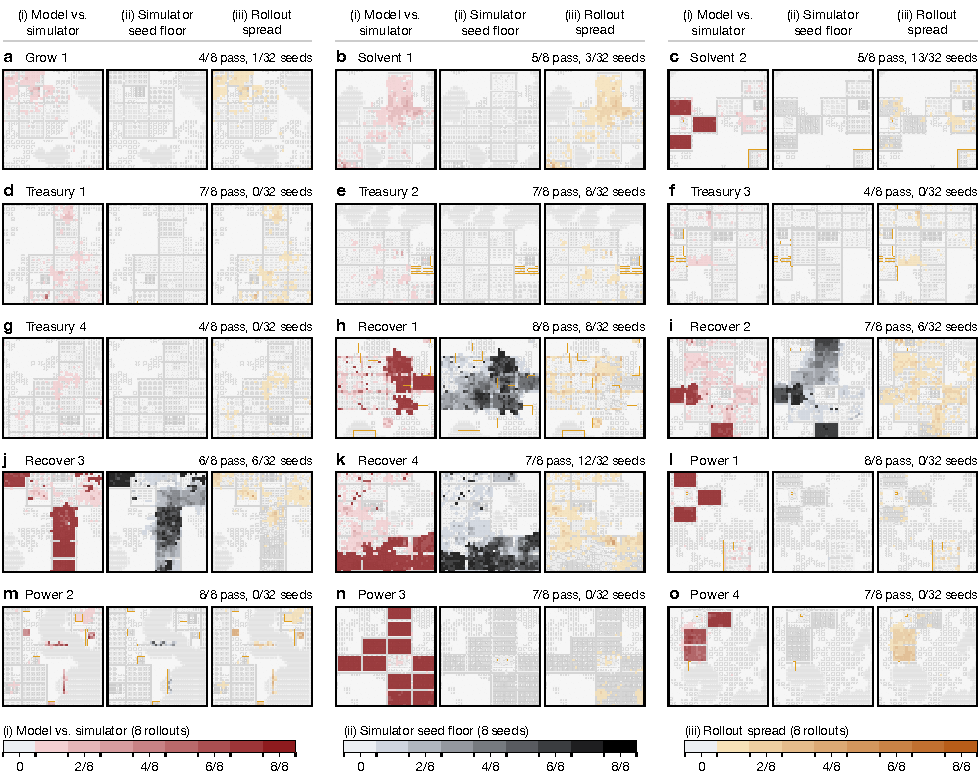
\includegraphics[width=\textwidth]{figures/fig_heatmaps.pdf}
\caption{\textbf{Spatial decomposition of world-model error, simulator stochasticity, and within-model rollout spread.} For each of the \GalPairs{} exploited city plans in Figure~\ref{fig:gallery} (matching panel letters and \GalCrop{}-by-\GalCrop{} spatial windows, overlaid on desaturated month-\Horizon{} procedural city sprites with gold outlines marking the plan's direct spatial build/demolish footprint), three per-tile heat maps show (i) \emph{Model vs.\ simulator} (share of \HeatSamples{} world-model rollouts diverging in tile class or power status from primary engine replay, crimson), (ii) \emph{Simulator seed floor} (share of \HeatSeeds{} independent engine seeds diverging from the primary seed in the exact simulator, charcoal), and (iii) \emph{Rollout spread} (internal disagreement across the \HeatSamples{} world-model rollouts, amber).}
\label{fig:heatmaps}
\end{figure*}


\subsection{Complete Benchmark Reference Tables}

Tables~\ref{tab:main}--\ref{tab:rl} provide the complete numerical records underlying Sections~\ref{sec:setting}--\ref{sec:coverage}, covering primary-model scaling across optimisers and budgets (Table~\ref{tab:main}), task-family breakdowns at $B ={}$\Bp{3} (Table~\ref{tab:family}), cross-ladder search curves across all \Ladder{} checkpoints (Table~\ref{tab:curves}), short-horizon fidelity (Table~\ref{tab:test}), \Horizon-month rollout drift and held-out ELBO (Table~\ref{tab:horizon}), threshold sensitivity on \emph{recover} (Table~\ref{tab:threshold}), and per-checkpoint PPO results (Table~\ref{tab:rl}).

\begin{table}[tbp]
\caption{Primary \SizeM{} world model paired against the exact-simulator reference across all \MainInstances{} core instances and the \WellPosed{} well-posed subset. ``False acceptance'' denotes selections accepted by the model and rejected by the \OracleSeeds-seed oracle; ``Exact ref.'' denotes the identical optimiser inside the exact-simulator reference, with the paired difference beside it; ``Truly passing'' gives ground-truth oracle pass share (model / exact reference); and ``False rej.'' gives the share of truly passing selections rejected by the judge (model / exact reference). Best-of-$N$ runs on twenty cities (\BonInstances{} instances). Bottom rows evaluate initial trajectories from \RlMonths{}-step PPO policies under the identical \KVerdict-sample verdict rule.}
\label{tab:main}
\centering\scriptsize\setlength{\tabcolsep}{3.5pt}
% Generated by paper/scripts/make_numbers.py from results/audit/ladder/os_50m_full/samples_006000000/tasks_v2_H24/reference.json and results/audit/ladder/os_50m_full/samples_006000000/tasks_v2_H24_cem_seeded/reference.json
\setlength{\tabcolsep}{1.2pt}
\begin{tabular*}{\textwidth}{@{\extracolsep{\fill}}llrlrlccrlc@{}}
\toprule
& & \multicolumn{6}{c}{All instances} & \multicolumn{3}{c}{Well posed} \\
\cmidrule(lr){3-8}\cmidrule(l){9-11}
Search & $B$ & $n$ & False acceptance & Exact ref. & Difference & Truly passing & False rej. & $n$ & Difference & Truly passing \\
\midrule
Random & $10^{0}$ & 193 & 0.083 {\tiny[0.051, 0.123]} & 0.021 & +0.062 {\tiny[+0.026, +0.103]} & 0.031/0.031 & 0.500/0.167 & 148 & +0.068 {\tiny[+0.028, +0.116]} & 0.027/0.027 \\
 & $10^{1}$ & 193 & 0.124 {\tiny[0.089, 0.167]} & 0.031 & +0.093 {\tiny[+0.048, +0.138]} & 0.140/0.223 & 0.333/0.023 & 148 & +0.095 {\tiny[+0.047, +0.146]} & 0.176/0.284 \\
 & $10^{2}$ & 193 & 0.130 {\tiny[0.085, 0.173]} & 0.057 & +0.073 {\tiny[+0.005, +0.128]} & 0.269/0.435 & 0.308/0.048 & 148 & +0.095 {\tiny[+0.032, +0.149]} & 0.318/0.527 \\
 & $10^{3}$ & 193 & 0.150 {\tiny[0.104, 0.195]} & 0.083 & +0.067 {\tiny[+0.010, +0.125]} & 0.311/0.492 & 0.317/0.053 & 148 & +0.081 {\tiny[+0.020, +0.147]} & 0.378/0.574 \\
\addlinespace[2pt]
Adaptive & $10^{1}$ & 193 & 0.109 {\tiny[0.072, 0.153]} & 0.026 & +0.083 {\tiny[+0.037, +0.130]} & 0.067/0.130 & 0.462/0.040 & 148 & +0.088 {\tiny[+0.049, +0.137]} & 0.088/0.162 \\
 & $10^{2}$ & 193 & 0.145 {\tiny[0.104, 0.189]} & 0.052 & +0.093 {\tiny[+0.037, +0.144]} & 0.192/0.347 & 0.324/0.090 & 148 & +0.101 {\tiny[+0.048, +0.162]} & 0.216/0.426 \\
 & $10^{3}$ & 193 & 0.181 {\tiny[0.130, 0.229]} & 0.067 & +0.114 {\tiny[+0.052, +0.173]} & 0.275/0.466 & 0.208/0.100 & 148 & +0.108 {\tiny[+0.048, +0.169]} & 0.331/0.574 \\
\addlinespace[2pt]
Best-of-$N$ & $10^{0}$ & 99 & 0.071 {\tiny[0.030, 0.117]} & 0.000 & +0.071 {\tiny[+0.030, +0.117]} & 0.091/0.091 & 0.111/0.000 & 81 & +0.062 {\tiny[+0.024, +0.120]} & 0.111/0.111 \\
 & $10^{1}$ & 99 & 0.141 {\tiny[0.081, 0.212]} & 0.040 & +0.101 {\tiny[+0.031, +0.172]} & 0.323/0.374 & 0.125/0.054 & 81 & +0.062 {\tiny[0.000, +0.143]} & 0.383/0.444 \\
 & $10^{2}$ & 99 & 0.152 {\tiny[0.081, 0.270]} & 0.051 & +0.101 {\tiny[+0.020, +0.227]} & 0.404/0.404 & 0.225/0.025 & 81 & +0.099 {\tiny[+0.012, +0.221]} & 0.481/0.494 \\
 & $10^{3}$ & 99 & 0.101 {\tiny[0.051, 0.172]} & 0.040 & +0.061 {\tiny[0.000, +0.141]} & 0.374/0.455 & 0.189/0.067 & 81 & +0.049 {\tiny[\mbox{-}0.013, +0.133]} & 0.444/0.543 \\
\addlinespace[2pt]
RL, main & $10^{6}$ m. & 579 & 0.178 {\tiny[0.137, 0.225]} & 0.056 & +0.122 {\tiny[+0.076, +0.175]} & 0.152/-- & -- & -- & -- & -- \\
RL, ladder & $10^{6}$ m. & 13,896 & 0.233 {\tiny[0.186, 0.284]} & 0.064 & +0.170 {\tiny[+0.124, +0.220]} & 0.141/-- & -- & -- & -- & -- \\
\bottomrule
\end{tabular*}

\end{table}

\begin{table}[tbp]
\caption{Task-family breakdown on the primary \SizeM{} checkpoint at $B ={}$\Bp{3} across all core instances and well-posed instances.}
\label{tab:family}
\centering\scriptsize\setlength{\tabcolsep}{3.5pt}
% Generated by paper/scripts/make_numbers.py from the two reference.json files of the main checkpoint
\setlength{\tabcolsep}{1.5pt}
\begin{tabular*}{\textwidth}{@{\extracolsep{\fill}}llrlrlccrlc@{}}
\toprule
& & \multicolumn{6}{c}{All instances} & \multicolumn{3}{c}{Well posed} \\
\cmidrule(lr){3-8}\cmidrule(l){9-11}
Task & Search & $n$ & False acceptance & Exact ref. & Difference & Accepted & Truly passing & $n$ & Difference & Truly passing \\
\midrule
grow & random & 40 & 0.025 {\tiny[0.000, 0.125]} & 0.100 & \mbox{-}0.075 {\tiny[\mbox{-}0.200, +0.025]} & 0.050/0.375 & 0.225/0.275 & 36 & \mbox{-}0.056 {\tiny[\mbox{-}0.167, +0.028]} & 0.250/0.306 \\
 & adaptive & 40 & 0.000 {\tiny[0.000, 0.072]} & 0.050 & \mbox{-}0.050 {\tiny[\mbox{-}0.150, 0.000]} & 0.050/0.300 & 0.150/0.275 & 36 & \mbox{-}0.056 {\tiny[\mbox{-}0.167, 0.000]} & 0.167/0.306 \\
\addlinespace[2pt]
solvent & random & 38 & 0.053 {\tiny[0.000, 0.158]} & 0.158 & \mbox{-}0.105 {\tiny[\mbox{-}0.263, +0.026]} & 0.053/0.421 & 0.026/0.289 & 20 & \mbox{-}0.050 {\tiny[\mbox{-}0.228, +0.100]} & 0.050/0.350 \\
 & adaptive & 38 & 0.053 {\tiny[0.000, 0.184]} & 0.026 & +0.026 {\tiny[\mbox{-}0.053, +0.132]} & 0.079/0.184 & 0.053/0.211 & 20 & 0.000 {\tiny[0.000, 0.000]} & 0.100/0.350 \\
\addlinespace[2pt]
treasury & random & 40 & 0.200 {\tiny[0.100, 0.350]} & 0.025 & +0.175 {\tiny[+0.050, +0.325]} & 0.350/0.525 & 0.250/0.525 & 39 & +0.179 {\tiny[+0.051, +0.333]} & 0.256/0.538 \\
 & adaptive & 40 & 0.275 {\tiny[0.150, 0.425]} & 0.075 & +0.200 {\tiny[+0.025, +0.375]} & 0.500/0.525 & 0.250/0.550 & 39 & +0.205 {\tiny[+0.026, +0.385]} & 0.256/0.564 \\
\addlinespace[2pt]
recover & random & 35 & 0.343 {\tiny[0.200, 0.514]} & 0.143 & +0.200 {\tiny[0.000, +0.400]} & 0.571/0.400 & 0.314/0.343 & 13 & +0.154 {\tiny[0.000, +0.462]} & 0.538/0.462 \\
 & adaptive & 35 & 0.371 {\tiny[0.229, 0.543]} & 0.200 & +0.171 {\tiny[\mbox{-}0.029, +0.343]} & 0.571/0.400 & 0.257/0.257 & 13 & +0.077 {\tiny[\mbox{-}0.154, +0.308]} & 0.385/0.385 \\
\addlinespace[2pt]
power & random & 40 & 0.150 {\tiny[0.050, 0.275]} & 0.000 & +0.150 {\tiny[+0.050, +0.275]} & 0.800/1.000 & 0.725/1.000 & 40 & +0.150 {\tiny[+0.050, +0.275]} & 0.725/1.000 \\
 & adaptive & 40 & 0.225 {\tiny[0.125, 0.375]} & 0.000 & +0.225 {\tiny[+0.125, +0.375]} & 0.800/1.000 & 0.650/1.000 & 40 & +0.225 {\tiny[+0.125, +0.375]} & 0.650/1.000 \\
\bottomrule
\end{tabular*}

\end{table}

\ifAcrossDone
\begin{table}[tbp]
\caption{Cross-model search audit across all \Ladder{} world-model checkpoints, reporting random shooting across all \AllCities{} cities ($B ={}$\Bp{1} to \Bp{3}) and adaptive CEM at $B ={}$\Bp{3} on the \HeldOutFamilies-city core benchmark\ifAcAdSet{} across \AcAdSetName{}\fi, pooled across the five task families.}
\label{tab:curves}
\centering\scriptsize\setlength{\tabcolsep}{3.5pt}
% Generated by paper/scripts/make_numbers.py from results/analysis/pairs.csv
\setlength{\tabcolsep}{2pt}
\begin{tabular*}{\textwidth}{@{\extracolsep{\fill}}llllccccccccc@{}}
\toprule
 & & & & \multicolumn{6}{c}{Random shooting (120 cities)} & \multicolumn{3}{c}{Adaptive CEM, $10^{3}$ (40-city core)} \\
\cmidrule(lr){5-10}\cmidrule(l){11-13}
Objective & Size & Data & Stage & $10^{1}$ & $10^{2}$ & $10^{3}$ & Excess & Truly passing & Exact ref. & False acc. & Excess & Truly passing \\
\midrule
one-step & 15M & full & half-trained & 0.103 & 0.132 & 0.120 & +0.051 & 0.375 & 0.070 & 0.192 & +0.124 & 0.233 \\
one-step & 15M & full & final & 0.120 & 0.131 & 0.153 & +0.084 & 0.362 & 0.070 & 0.192 & +0.124 & 0.275 \\
one-step & 15M & small & half-trained & 0.120 & 0.134 & 0.146 & +0.077 & 0.334 & 0.070 & 0.264 & +0.197 & 0.181 \\
one-step & 15M & small & final & 0.117 & 0.143 & 0.139 & +0.070 & 0.343 & 0.070 & 0.249 & +0.181 & 0.192 \\
one-step & 50M & full & half-trained & 0.125 & 0.122 & 0.108 & +0.038 & 0.366 & 0.070 & 0.202 & +0.135 & 0.181 \\
one-step & 50M & full & final & 0.138 & 0.138 & 0.162 & +0.092 & 0.336 & 0.070 & 0.181 & +0.114 & 0.275 \\
one-step & 50M & small & half-trained & 0.153 & 0.176 & 0.166 & +0.096 & 0.352 & 0.070 & 0.238 & +0.171 & 0.228 \\
one-step & 50M & small & final & 0.176 & 0.209 & 0.232 & +0.162 & 0.328 & 0.070 & 0.285 & +0.218 & 0.202 \\
one-step & 100M & full & half-trained & 0.129 & 0.145 & 0.145 & +0.075 & 0.355 & 0.070 & 0.223 & +0.155 & 0.238 \\
one-step & 100M & full & final & 0.096 & 0.092 & 0.110 & +0.040 & 0.345 & 0.070 & 0.140 & +0.073 & 0.269 \\
one-step & 100M & small & half-trained & 0.153 & 0.167 & 0.155 & +0.085 & 0.328 & 0.070 & 0.238 & +0.171 & 0.181 \\
one-step & 100M & small & final & 0.160 & 0.167 & 0.186 & +0.117 & 0.336 & 0.070 & 0.311 & +0.244 & 0.202 \\
pushforward & 15M & full & half-trained & 0.298 & 0.328 & 0.310 & +0.240 & 0.307 & 0.070 & 0.332 & +0.264 & 0.238 \\
pushforward & 15M & full & final & 0.232 & 0.265 & 0.272 & +0.202 & 0.291 & 0.070 & 0.275 & +0.207 & 0.254 \\
pushforward & 15M & small & half-trained & 0.166 & 0.174 & 0.153 & +0.084 & 0.343 & 0.070 & 0.269 & +0.202 & 0.181 \\
pushforward & 15M & small & final & 0.118 & 0.129 & 0.113 & +0.044 & 0.341 & 0.070 & 0.197 & +0.130 & 0.187 \\
pushforward & 50M & full & half-trained & 0.193 & 0.232 & 0.214 & +0.145 & 0.345 & 0.070 & 0.244 & +0.176 & 0.202 \\
pushforward & 50M & full & final & 0.183 & 0.188 & 0.188 & +0.118 & 0.321 & 0.070 & 0.249 & +0.181 & 0.181 \\
pushforward & 50M & small & half-trained & 0.179 & 0.204 & 0.186 & +0.117 & 0.315 & 0.070 & 0.259 & +0.192 & 0.181 \\
pushforward & 50M & small & final & 0.152 & 0.176 & 0.172 & +0.103 & 0.319 & 0.070 & 0.228 & +0.161 & 0.228 \\
pushforward & 100M & full & half-trained & 0.181 & 0.207 & 0.207 & +0.138 & 0.373 & 0.070 & 0.218 & +0.150 & 0.295 \\
pushforward & 100M & full & final & 0.155 & 0.192 & 0.190 & +0.120 & 0.336 & 0.070 & 0.192 & +0.124 & 0.275 \\
pushforward & 100M & small & half-trained & 0.120 & 0.152 & 0.134 & +0.064 & 0.310 & 0.070 & 0.218 & +0.150 & 0.192 \\
pushforward & 100M & small & final & 0.111 & 0.139 & 0.122 & +0.052 & 0.329 & 0.070 & 0.187 & +0.119 & 0.218 \\
\bottomrule
\end{tabular*}

\end{table}
\fi

\begin{table}[tbp]
\caption{Short-horizon trajectory fidelity across all \TestRuns{} completed training runs on the held-out test split (\TestTransitions{} transitions, \TestPlans{} trajectories), reporting one-month structural (and raw) changed-tile F1, \RollA-month changed-since-start structural F1, and median relative population and treasury errors. Non-zero seeds denote the additional \SizeM{} ensemble runs. \HorizonTableNote{}}
\label{tab:test}
\centering\scriptsize\setlength{\tabcolsep}{4pt}
% Generated by paper/scripts/make_numbers.py from results/fidelity/ladder/<run>/test/<run>_samples_<final>_dec-a.json
\setlength{\tabcolsep}{3pt}
\begin{tabular*}{\textwidth}{@{\extracolsep{\fill}}llllccccc@{}}
\toprule
Objective & Size & Data & Seed & F1, 1 m & Raw F1, 1 m & F1, 12 m & Pop., 12 m & Funds, 12 m \\
\midrule
one-step & 15M & small & 0 & 0.170 & 0.287 & 0.369 & 0.057 & 0.046 \\
pushforward & 15M & small & 0 & 0.147 & 0.256 & 0.295 & 0.052 & 0.063 \\
one-step & 15M & full & 0 & 0.169 & 0.282 & 0.373 & 0.052 & 0.048 \\
pushforward & 15M & full & 0 & 0.153 & 0.263 & 0.308 & 0.053 & 0.060 \\
one-step & 50M & small & 0 & 0.166 & 0.287 & 0.372 & 0.045 & 0.038 \\
pushforward & 50M & small & 0 & 0.148 & 0.259 & 0.304 & 0.056 & 0.038 \\
one-step & 50M & full & 0 & 0.179 & 0.294 & 0.372 & 0.060 & 0.035 \\
pushforward & 50M & full & 0 & 0.168 & 0.282 & 0.319 & 0.050 & 0.034 \\
one-step & 100M & small & 0 & 0.172 & 0.297 & 0.376 & 0.052 & 0.034 \\
pushforward & 100M & small & 0 & 0.155 & 0.273 & 0.290 & 0.061 & 0.039 \\
one-step & 100M & full & 0 & 0.178 & 0.294 & 0.379 & 0.048 & 0.030 \\
pushforward & 100M & full & 0 & 0.168 & 0.280 & 0.338 & 0.044 & 0.027 \\
one-step & 50M & full & 1 & 0.182 & 0.294 & 0.382 & 0.048 & 0.034 \\
pushforward & 50M & full & 1 & 0.168 & 0.282 & 0.329 & 0.044 & 0.038 \\
one-step & 50M & full & 2 & 0.178 & 0.295 & 0.376 & 0.050 & 0.036 \\
pushforward & 50M & full & 2 & 0.172 & 0.286 & 0.323 & 0.046 & 0.056 \\
\midrule
\multicolumn{4}{@{}l}{Engine under another seed} & 0.206 & 0.319 & 0.423 & 0.027 & 0.003 \\
\multicolumn{4}{@{}l}{Copy-last-state} & 0.000 & 0.000 & 0.000 & 0.112 & 0.400 \\
\bottomrule
\end{tabular*}

\end{table}

\begin{table}[tbp]
\caption{Long-horizon rollout drift at the \Horizon-month task horizon and held-out variational log-likelihood (ELBO in nats/transition on the development split at mid-training and full budget) across all final checkpoints and the coverage-retrained model.}
\label{tab:horizon}
\centering\scriptsize\setlength{\tabcolsep}{3.5pt}
% Generated by paper/scripts/make_numbers.py from results/analysis/fidelity_horizon.json and heldout_likelihood.json
\setlength{\tabcolsep}{2pt}
\begin{tabular*}{\textwidth}{@{\extracolsep{\fill}}llllrrrrrrc@{}}
\toprule
Objective & Size & Data & Seed & Overlays $\geq$ copy & Pollution & Fire cov. & Powered zones & ELBO, half & ELBO, final & Final below half \\
\midrule
one-step & 15M & small & 0 & 4 & 1.455 & 0.989 & 2.4 & \mbox{-}2948 & \mbox{-}3061 & yes \\
pushforward & 15M & small & 0 & 7 & 1.673 & 1.713 & 9.7 & \mbox{-}3000 & \mbox{-}3063 & yes \\
one-step & 15M & full & 0 & 5 & 1.530 & 1.017 & 2.8 & \mbox{-}2928 & \mbox{-}2779 & no \\
pushforward & 15M & full & 0 & 7 & 1.646 & 1.780 & 7.7 & \mbox{-}2843 & \mbox{-}2822 & no \\
one-step & 50M & small & 0 & 4 & 1.351 & 0.955 & 3.4 & \mbox{-}2952 & \mbox{-}3414 & yes \\
pushforward & 50M & small & 0 & 7 & 1.704 & 1.277 & 9.8 & \mbox{-}3159 & \mbox{-}3316 & yes \\
one-step & 50M & full & 0 & 6 & 1.520 & 1.127 & 6.1 & \mbox{-}2771 & \mbox{-}2664 & no \\
pushforward & 50M & full & 0 & 7 & 1.807 & 1.594 & 8.7 & \mbox{-}2719 & \mbox{-}2701 & no \\
one-step & 100M & small & 0 & 4 & 1.270 & 0.814 & 2.7 & \mbox{-}2905 & \mbox{-}3665 & yes \\
pushforward & 100M & small & 0 & 7 & 1.698 & 1.232 & 11.0 & \mbox{-}3280 & \mbox{-}3514 & yes \\
one-step & 100M & full & 0 & 6 & 1.546 & 1.180 & 7.9 & \mbox{-}2705 & \mbox{-}2574 & no \\
pushforward & 100M & full & 0 & 5 & 1.731 & 1.067 & 4.4 & \mbox{-}2626 & \mbox{-}2604 & no \\
one-step & 50M & full & 1 & 2 & 1.377 & 0.814 & 2.2 & \mbox{-}2780 & \mbox{-}2662 & no \\
pushforward & 50M & full & 1 & 7 & 1.745 & 3.591 & 8.9 & \mbox{-}2718 & \mbox{-}2700 & no \\
one-step & 50M & full & 2 & 6 & 1.577 & 1.088 & 6.6 & \mbox{-}2772 & \mbox{-}2666 & no \\
pushforward & 50M & full & 2 & 7 & 1.893 & 9.291 & 7.1 & \mbox{-}2725 & \mbox{-}2704 & no \\
one-step & 50M & full + cov. & 0 & 7 & 1.552 & 1.197 & 4.0 & \mbox{-}2786 & \mbox{-}2664 & no \\
\midrule
\multicolumn{4}{@{}l}{Engine under another seed} & & 0.703 & 0.125 & 0.0 & & & \\
\multicolumn{4}{@{}l}{Copy-last-state} & & 1.000 & 1.000 & 0.5 & & & \\
\bottomrule
\end{tabular*}

\end{table}

\begin{table}[tbp]
\caption{Target-threshold sensitivity on \emph{recover} for random shooting at $B ={}$\Bp{3} on the primary checkpoint, re-evaluated exactly at thresholds set one quarter, one half, and three quarters of the way between the best constant no-build plan ($c$) and the engine-search ceiling ($e$).}
\label{tab:threshold}
\centering\scriptsize\setlength{\tabcolsep}{3.5pt}
% Generated by paper/scripts/make_numbers.py from results/analysis/threshold_reread.json
\setlength{\tabcolsep}{3pt}
\begin{tabular*}{\textwidth}{@{\extracolsep{\fill}}lrlrlcc@{}}
\toprule
Threshold $\lambda$ (from $c$ to $e$) & $n$ & False acceptance & Exact ref. & Excess & Truly passing, model/ref. & World model accepts \\
\midrule
$0.25$ & 35 & 0.257 {\tiny[0.143, 0.429]} & 0.200 & +0.057 {\tiny[\mbox{-}0.114, +0.229]} & 0.514 / 0.486 & 0.657 \\
$0.50$ (benchmark) & 35 & 0.343 {\tiny[0.200, 0.514]} & 0.143 & +0.200 {\tiny[0.000, +0.400]} & 0.314 / 0.343 & 0.571 \\
$0.75$ & 35 & 0.400 {\tiny[0.257, 0.571]} & 0.171 & +0.229 {\tiny[0.000, +0.429]} & 0.143 / 0.143 & 0.486 \\
\bottomrule
\end{tabular*}

\end{table}

\begin{table}[tbp]
\caption{In-imagination PPO performance across all \RlCkptsDone{} world-model checkpoints after \RlMonths{} imagined steps (means over five task families and three seeds per cell, with engine-trained PPO reference optimism gap \RlEngGap{} \ci{\RlEngGapCI}).}
\label{tab:rl}
\centering\scriptsize\setlength{\tabcolsep}{4pt}
% Generated by paper/scripts/make_numbers.py from results/rl/<checkpoint>__<family>__s<seed>__tasks_v2_H24/eval3_001000000.summary.json
\setlength{\tabcolsep}{2.5pt}
\begin{tabular*}{\textwidth}{@{\extracolsep{\fill}}llllrccccc@{}}
\toprule
Objective & Size & Data & Stage & Runs & Dream accepts & Oracle accepts & Gap & Closed loop & Margin inflation \\
\midrule
one-step & 15M & full & half-trained & 15 & 0.282 & 0.181 & +0.101 & 0.255 & +0.007 \\
one-step & 15M & full & final & 15 & 0.285 & 0.167 & +0.118 & 0.233 & \mbox{-}0.017 \\
one-step & 15M & small & half-trained & 15 & 0.291 & 0.148 & +0.143 & 0.219 & +0.012 \\
one-step & 15M & small & final & 15 & 0.253 & 0.129 & +0.123 & 0.201 & \mbox{-}0.084 \\
one-step & 50M & full & half-trained & 15 & 0.327 & 0.159 & +0.168 & 0.223 & +0.097 \\
one-step & 50M & full & final & 15 & 0.271 & 0.138 & +0.133 & 0.202 & \mbox{-}0.016 \\
one-step & 50M & small & half-trained & 15 & 0.366 & 0.151 & +0.215 & 0.223 & +0.221 \\
one-step & 50M & small & final & 15 & 0.346 & 0.147 & +0.199 & 0.216 & +0.170 \\
one-step & 100M & full & half-trained & 15 & 0.330 & 0.167 & +0.162 & 0.242 & +0.111 \\
one-step & 100M & full & final & 15 & 0.211 & 0.141 & +0.070 & 0.192 & \mbox{-}0.177 \\
one-step & 100M & small & half-trained & 15 & 0.322 & 0.161 & +0.161 & 0.216 & +0.141 \\
one-step & 100M & small & final & 15 & 0.294 & 0.144 & +0.150 & 0.209 & +0.029 \\
pushforward & 15M & full & half-trained & 15 & 0.486 & 0.135 & +0.351 & 0.202 & +0.287 \\
pushforward & 15M & full & final & 15 & 0.433 & 0.128 & +0.305 & 0.187 & +0.190 \\
pushforward & 15M & small & half-trained & 15 & 0.342 & 0.128 & +0.214 & 0.181 & \mbox{-}0.010 \\
pushforward & 15M & small & final & 15 & 0.265 & 0.126 & +0.140 & 0.163 & \mbox{-}0.203 \\
pushforward & 50M & full & half-trained & 15 & 0.411 & 0.139 & +0.272 & 0.203 & +0.215 \\
pushforward & 50M & full & final & 15 & 0.380 & 0.119 & +0.261 & 0.162 & +0.251 \\
pushforward & 50M & small & half-trained & 15 & 0.316 & 0.128 & +0.188 & 0.196 & \mbox{-}0.023 \\
pushforward & 50M & small & final & 15 & 0.261 & 0.114 & +0.147 & 0.172 & \mbox{-}0.175 \\
pushforward & 100M & full & half-trained & 15 & 0.384 & 0.155 & +0.229 & 0.216 & +0.163 \\
pushforward & 100M & full & final & 15 & 0.337 & 0.142 & +0.195 & 0.205 & +0.104 \\
pushforward & 100M & small & half-trained & 15 & 0.246 & 0.121 & +0.125 & 0.168 & \mbox{-}0.273 \\
pushforward & 100M & small & final & 15 & 0.223 & 0.115 & +0.108 & 0.158 & \mbox{-}0.338 \\
\bottomrule
\end{tabular*}

\end{table}

\subsection{Additional Modeling, Search, and Controller Ablations}\label{app:ablations}

\emph{Pushforward rollout fine-tuning versus one-step variational training.} Fine-tuning final one-step models on stop-gradient posterior-mode rollouts slightly lowers one-month structural changed-tile F1 in \SfLowerOne{} of \SfPairs{} parent-child pairs and \RollA-month changed-since-start F1 in \SfLowerTwelve{} of \SfPairs{} pairs (primary lineage shifts from \TestMainFTwelve{} to \SfMainFTwelve{}), because in a stochastic cellular automaton whose own cross-seed changed-tile F1 is \TestFloorFOne{}, pairing a rolled-out model state against a single archived engine state injects transition variance; both model families remain in our \Ladder-checkpoint ladder.

\emph{Unseeded column-independent CEM versus seeded elite-mutation CEM.} Standard unseeded CEM \citep{deboer2005cem}, which resamples all \PlanColumns{} action columns independently from fitted marginals at each generation, disrupts multi-month spatial coordination, so even inside the exact-simulator reference at $B ={}$\Bp{3}, unseeded CEM achieves only \PerfCemThouOrAcc{} ground-truth success versus \PerfRandThouOrAcc{} for random shooting (with the primary world model accepting \CemThouJudgeAcc{} of its own unseeded selections), motivating our logged-plan-seeded elite-mutation CEM in Section~\ref{sec:pressure}.

\emph{Shuffled-residual noise surrogates.} Replacing the world model with a synthetic surrogate that adds shuffled empirical model residuals to ground-truth margins (passing exact-simulator calibration across all \AcceptVolGroups{} of \AcceptVolGroups{} budget cells in volatility-matched form) yields \RandThouVolFloor{} false acceptance under \Bp{3} random shooting (\RandThouPlainFloor{} unweighted), exceeding the actual neural model's \RandThouHack{} because smooth state-dependent model biases preserve local plan rankings better than i.i.d.\ residual draws.

\emph{Internal accounting drift as an unsupervised anomaly signal.} Checking whether imagined trajectories violate exact municipal budget conservation by more than \BreachShare{} per cent of initial funds shows breach rates rising across random-shooting budgets (\TrRandOne{}, \TrRandTen{}, \TrRandHund{}, and \TrRandThou{} from \Bp{0} to \Bp{3} among accepted plans, vs.\ \TrRandThouRej{} on rejected plans and \TrBeh{} on unoptimised logged plans), yet separates false acceptances (\TrSplitWrong{}) from true acceptances (\TrSplitRight{}, difference \TrSplitDiff{} \ci{\TrSplitDiffCI}, rejected \TrSplitRej{}) too weakly to serve as a standalone filter.

\emph{Behaviour-cloned warm-starting and hysteresis-free replanning.} Warm-starting PPO spatial heads from scripted builders improved engine-side returns on \emph{power} (\RlHybridDiffPower{} \ci{\RlHybridDiffPowerCI}) and \emph{solvent} (\RlHybridDiffSolv{} \ci{\RlHybridDiffSolvCI}) with neutral effects elsewhere, so we report uniform from-scratch PPO throughout. Similarly, inside the exact simulator, naive monthly replanners without switching hysteresis (either redrawing fresh proposals each month without retaining the incumbent, passing \RpVOneReplan{} vs.\ \RpVOneOpen{} of \RpVOneN{} overall and \RpVOnePowerReplan{} vs.\ \RpVOnePowerOpen{} of \RpVOnePowerN{} on \emph{power}, or pooling the incumbent without a standard-error switching margin, passing \RpVTwoReplan{} vs.\ \RpVTwoOpen{} of \RpVTwoN{} overall, \RpVTwoGrowReplan{} vs.\ \RpVTwoGrowOpen{} of \RpVTwoGrowN{} on \emph{grow}, and \RpVTwoRecovReplan{} vs.\ \RpVTwoRecovOpen{} of \RpVTwoRecovN{} on \emph{recover}) thrash between incompatible spatial build plans, motivating the \RpSwitchSe{}-standard-error hysteresis gate used in Section~\ref{sec:replan}.

\section{Domain-General Audit Library and Continuous-Control Check}\label{app:external}

% Verified against hpr-dream/ source signatures by protocols.instrument() in paper/scripts/protocols.py.
All search audits and statistical estimators are implemented in \hpd{}, a domain-agnostic Python library depending solely on \texttt{numpy} and \texttt{scipy}. It represents multi-step plans as integer arrays over a typed schema of categorical and bounded-integer columns, interfaces with any candidate world model via a batch scoring callback and with ground truth via an oracle margin callback, and logs standardised per-selection audit records (instance, city cluster, optimiser, budget, seed, plan hash, model pass share, and ground-truth verdict). Environment-specific adaptors handle rollout execution, with our Micropolis adaptor wrapping both neural checkpoints and the fresh-seed exact-simulator reference and our continuous-control adaptor snapshotting and restoring MuJoCo simulator states for TD-MPC2. From these callbacks, \hpd{} executes random shooting, best-of-$N$, standard CEM, and seeded adaptive CEM under exact call-budget accounting, and computes city-clustered percentile and BCa bootstrap intervals, exact zero-event upper bounds, false acceptance, conditional and false rejection, paired reference excesses, Brier and log-score decompositions, ROC AUC, clustered Spearman and Kendall rank correlations, shuffled-residual and binary-flip noise surrogates, and structured JSON audit cards.


To verify that \hpd{} operates cleanly out-of-the-box on external latent-space world models we did not train, we audited two publicly released single-task TD-MPC2 checkpoints \citep{hansen2024tdmpc2,tdmpc2checkpoints} on DeepMind Control Suite tasks \citep{tunyasuvunakool2020dmcontrol}. Here the world model comprises TD-MPC2's learned encoder, latent transition dynamics, and reward head, while the oracle replays continuous action sequences from exactly restored MuJoCo physics states (numerical state-restoration tolerance \ExtOracleTolerance{}). Across \ExtStarts{} initial states per task, thresholds over \ExtHorizon-step open-loop trajectories are calibrated so \ExtAccLo{}--\ExtAccHi{} of correlated random behaviour plans pass; because MuJoCo replay is deterministic, the exact-simulator false-acceptance floor is identically zero. Because TD-MPC2 trains on short \ExtMppiHorizon-step rollouts bootstrapped with terminal value estimates rather than open-loop \ExtHorizon-step sums, unrolling its latent reward head open loop over \ExtHorizon{} steps induces a strong upward return bias of \WalkerResid{} to \CheetahResid{} logged-plan standard deviations, falsely accepting \CheetahFp{} (\emph{cheetah-run}) and \WalkerFp{} (\emph{walker-walk}) of failing behaviour plans. Consequently, open-loop shooting actually lowers unconditional false acceptance from \CheetahRandOneHack{} and \WalkerRandOneHack{} at $B ={}$\Bp{0} to \CheetahRandThouHack{} \ci{\CheetahRandThouHackCI} and \WalkerRandThouHack{} \ci{\WalkerRandThouHackCI} at $B ={}$\Bp{3} as genuinely higher-return trajectories are selected (running TD-MPC2's native MPPI planner open loop with \CheetahMppiB{} rollouts yields \CheetahMppiHack{} and \WalkerMppiHack{} false acceptance; \emph{hopper-hop} was excluded because \HopperZeroStarts{} of \ExtStarts{} starts yielded identically zero behaviour return). We treat this purely as an external software validation rather than a claim about model-predictive control when TD-MPC2 is run closed loop at its native \ExtMppiHorizon-step horizon.

\paragraph{Code, data, and licensing.}
\hpd{} is released under the Apache-2.0 licence. The Micropolis C++ engine modifications, Python replay bindings, data generator, task harness, and evaluation scripts link against MicropolisCore and are released under GPL-3.0 with Electronic Arts' additional terms, with all modifications explicitly marked. Complete JSON/CSV result records, calibrated task definitions, figure scripts, and paper sources reproducing all numbers and graphics in this work are released under CC BY 4.0 via hyperprior.net. As noted in Appendix~\ref{app:emulator}, neural network checkpoints (documented by SHA-256 digest) and trained RL policies are not distributed.

\section{Extended Related Work}\label{app:morerelated}

\paragraph{Offline model-based optimisation and surrogate exploitation.}
Optimising static designs against learned reward surrogates produces severe out-of-distribution overestimation in offline model-based optimisation (MBO), motivating conservative conditioning, autofocused retraining, and adversarial regularisation across Design-Bench \citep{brookes2019cbas,fannjiang2020autofocused,kumar2020mins,trabucco2021coms,trabucco2022designbench}. Our setting extends static surrogate optimisation to autoregressive \Horizon-step stochastic dynamics where spatial actions compound nonlinearly and exact simulator replay benchmarks excess error over regressional Goodhart selection noise \citep{manheim2018goodhart,bailey2017pbo,ma2026selectiontax,bastani2026winners,eshwar2026proofcarrying} induced by structural dynamics errors \citep{pan2022misspecification,skalse2022gaming,jakobi1995noise,koos2013transferability}. In reward-model scaling for language and control agents, proxy-gold gaps grow predictably with KL divergence and optimisation budget \citep{gao2023scaling,frick2024ppe,kim2025rethinking,wen2025rethinking}.

\paragraph{Uncertainty regularisation, rollout fidelity, and generative game engines.}
Ensemble disagreement penalties \citep{kurutach2018metrpo,chua2018pets,yu2020mopo}, absorbing OOD halts \citep{kidambi2020morel}, value conservatism \citep{yu2021combo,rigter2022rambo}, and multi-step hallucinated or pushforward training \citep{talvitie2014regularization,talvitie2017selfcorrecting,venkatraman2015dad,brandstetter2022mpnpde} aim to bound rollout exploitation, though empirical correlations between ensemble variance and true dynamics error are often weak \citep{lu2022revisiting}. Recent preprints and benchmarks document reward inflation and dream-reality gaps in robotic and game world models \citep{jiang2026wovr,zhou2026wovrplus,khassanov2026lies,kieto2026moba,bhamidipaty2026renew,amd2026learningtofail,xu2026curewm,yang2026mirabench,reka2026worldmodelgym,kong2026tif,guzel2026prowl,odyssey2026prowl1} alongside off-policy world-model evaluation on fixed policy sets \citep{fu2021dope,zhang2021autoregressive} and interventional rollout debugging \citep{yao2026rolloutfaith,rahmani2026debugging,zhu2026dualfrontier,vakalis2026intervention}. Finally, our testbed builds on Micropolis RL environments \citep{earle2020gymcity} and complements neural game and strategy simulators spanning Atari, Doom, platformers, StarCraft~II, and turn-based strategy \citep{kaiser2020simple,micheli2023iris,alonso2024diamond,valevski2025gamengen,bruce2024genie,synnaeve2018defogger,egorov2022mamba,bamford2020nge,dyer2024interventionally,zhang2024marie,zhang2026starwm,li2026civworldbench}.
